\documentclass{article}

\usepackage[final]{neurips_2026}

\usepackage[utf8]{inputenc}
\usepackage[T1]{fontenc}
\usepackage{hyperref}
\usepackage{url}
\usepackage{booktabs}
\usepackage{amsfonts}
\usepackage{amsmath}
\usepackage{amssymb}
\usepackage{nicefrac}
\usepackage{microtype}
\usepackage{graphicx}
\usepackage{algorithm}
\usepackage{algorithmic}
\usepackage{subcaption}
\usepackage{xcolor}
\usepackage{tikz}
\usetikzlibrary{arrows.meta, positioning, fit, backgrounds, calc}
\usepackage{enumitem}

\newcommand{\ie}{\textit{i.e.}}
\newcommand{\eg}{\textit{e.g.}}
\newcommand{\cf}{\textit{cf.}}
\newcommand{\etal}{\textit{et al.}}

\title{The Alignment Hazard: Anti-Pareto Failure of Inference-Time Policy Composition on Directional Action Manifolds}

\author{Julian Quick\thanks{\texttt{juqu@dtu.dk}} \\ Marcus Binder Nilsen \\
DTU Wind Energy, Technical University of Denmark}

\begin{document}

\maketitle

\begin{abstract}
Long-horizon load and lifetime-fatigue budgets are most accurately modelled as \emph{anytime constraints}~\citep{mcmahan2024anytime}---budgets that must not be exceeded at any time, almost surely---and are typically slack within any single episode.
A natural inference-time approach to such budgets composes a pre-trained performance policy $\pi_{\mathrm{perf}}$ with a safety controller $\pi_{\mathrm{safe}}$ via $a=(1-\sigma)\pi_{\mathrm{perf}} + \sigma\pi_{\mathrm{safe}}$, where $\sigma\in[0,1]$ is paced by a budget urgency ratio in the style of optimal execution~\citep{almgren2001optimal} or reservoir water-value control~\citep{tilmant2008water, you2008hedging}.
We identify a failure mode of this scheme on \emph{directional action manifolds} that the inference-time composition literature does not address: when the controllers act on opposite sides of a non-convex cost ridge, the linear midpoint can have cost strictly higher than either endpoint---the schedule is \emph{anti-Pareto in $\sigma$}.
We demonstrate this directly in two domains.
In wind-farm yaw control with a blade-flap DEL surrogate~\citep{guillore2024sectoravg}, a direct $\sigma$-sweep at fixed $\pi_{\mathrm{perf}}$ (DEL-aware actor, yaw $\approx -15^\circ$) and $\pi_{\mathrm{safe}}$ (a $+7.5^\circ$ setpoint where DEL is low) shows a DEL peak at $\sigma=0.4$ that is $+212$ (3$\sigma$) and $+583$ (8$\sigma$) above the $\sigma\!=\!0$ and $\sigma\!=\!1$ endpoints respectively (\cref{fig:sigma_sweep}, $n=50$ episodes).
On Safety Gymnasium PointGoal1 the effect is much larger ($C\!=\!483$ at the worst-case rotation vs endpoints $C\!\le\!45$, \cref{tab:sg_hazard}).
We call this the \textbf{alignment hazard}, give a sufficient condition for cost-monotonicity (cost convex along the segment $\pi_{\mathrm{perf}}\to\pi_{\mathrm{safe}}$), and demonstrate the phenomenon empirically in two domains.
On wind-farm yaw control with a physics-grounded blade-flap DEL surrogate~\citep{guillore2024sectoravg}, a direct $\sigma$-sweep ($n=50$ episodes, $\pi_{\mathrm{safe}}=+7.5^\circ$ where DEL is low at both ends) gives a midpoint DEL ($63264$ at $\sigma\!=\!0.4$) strictly above both endpoints ($63052$, $62681$), with $3\sigma$ and $8\sigma$ separations respectively (\cref{fig:sigma_sweep}).
On Safety Gymnasium PointGoal1, rotating the safety controller's direction by $3\pi/4$ exposes the same failure: linear blend cost $C=483$, near-zero goal reward $R=0.5$.
We propose two cost-monotone fixes implemented with one extra cost probe per step: \textbf{rejection blending} (engage $\sigma$ only if the probe confirms $\pi_{\mathrm{safe}}$ helps) and \textbf{argmin selection} (binary commitment).
Both are provably no-worse-than-$\pi_{\mathrm{perf}}$.
Empirically they recover the Pareto frontier the linear blend misses: at the zero-crossing hazard regime on multi\_modal, rejection blending gains $+6.8\%$ farm power and $-0.6\%$ DEL versus linear (Table~\ref{tab:fix_recovery_zero}); on Safety Gymnasium at the worst-case rotation, $-97\%$ cost and $55\!\times$ reward (Table~\ref{tab:sg_hazard}).
A cross-layout ablation rules out the obvious objection ``just retrain with a DEL-aware reward'': $\beta\!=\!1$ DEL-aware training gives Pareto-improving behaviour on one layout and a $+5$--$7\%$ DEL trade-off on another, so deployment-time pacing remains required when retraining for every constraint is infeasible.
\end{abstract}

%----------------------------------------------------------------------
\section{Introduction}
\label{sec:intro}
%----------------------------------------------------------------------

\textbf{Scenario.}
A wind-farm operator deploys an RL controller for coordinated yaw wake steering; it was trained unconstrained and works well.
A new constraint arrives: per-turbine blade-flap fatigue must stay within a yearly budget tied to bearing-replacement schedules.
Retraining the controller for each new budget target is expensive; the operator already has a conservative yaw setpoint table.

\textbf{An instance of an old problem class.}
Long-horizon lifetime budgets are formalised as \emph{anytime constraints}~\citep{mcmahan2024anytime}: cumulative cost may not exceed the budget at any time, almost surely.
The same structure has been studied for decades in reservoir and hydropower operation~\citep{tilmant2008water, you2008hedging}, where the dual price on stored water (``water value'') is computed via stochastic programming and determines release decisions.
This paper does not introduce that problem class; it studies one inference-time approach to it, and a sharp failure mode of that approach.
A natural fix to deploy is to \emph{blend the two existing controllers at inference}, $a_t = (1-\sigma_t)\pi_{\mathrm{perf}} + \sigma_t\pi_{\mathrm{safe}}$, pacing $\sigma_t$ against the budget using the urgency intuition from optimal execution~\citep{almgren2001optimal}.
We show this natural fix has a sharp failure mode on directional action manifolds, and propose a cheap, provably cost-monotone replacement.

\textbf{The alignment hazard.}
Yaw is a directional setpoint on a manifold, not a scalar utility.
Blade-flap damage-equivalent load (DEL) peaks when the rotor is aligned with the wind, drops on either side of misalignment, and recovers at large magnitudes.
When $\pi_{\mathrm{perf}}$ yaws negative and $\pi_{\mathrm{safe}}$ yaws positive, the linear midpoint $\sigma=0.5$ produces \emph{zero yaw}---the cost maximum.
A direct $\sigma$-sweep at fixed controllers ($n=50$ episodes per $\sigma$) confirms the prediction: cumulative DEL peaks mid-segment, strictly above both endpoints at $3\sigma$ and $8\sigma$ of the standard error (\Cref{fig:sigma_sweep}).
We name this the \textbf{alignment hazard} and show in \Cref{sec:monotone_theory} that it arises whenever cost is non-convex along the segment $\pi_{\mathrm{perf}}\!\to\!\pi_{\mathrm{safe}}$.
On Safety Gymnasium PointGoal1 with a rotated artificial-potential-field controller (\Cref{fig:alignment_hazard}b), the same phenomenon shows up as a $10\times$ cost spike and near-zero reward at intermediate rotations.

\textbf{The fix.}
We propose two cost-monotone replacements for the linear blend.
\textbf{Rejection blending} engages $\sigma$ only when a per-step cost probe confirms $\pi_{\mathrm{safe}}$ helps; \textbf{argmin selection} commits to whichever of $\{\pi_{\mathrm{perf}}, \pi_{\mathrm{safe}}\}$ has lower 1-step probe cost.
Both require one extra cost evaluation per step (a surrogate forward pass or critic call) and are provably no-worse-than-$\pi_{\mathrm{perf}}$.
Empirically they recover the Pareto frontier the linear blend collapses: at the zero-crossing hazard ($y^{\mathrm{tgt}}=0$) on multi\_modal, rejection blending gains $+6.8\%$ power and $-0.6\%$ DEL versus linear; on Safety Gymnasium at the worst-case rotation, $C\!=\!15$ vs $C\!=\!483$ and $R\!=\!27$ vs $R\!=\!0.5$.

\textbf{What about ``just retrain''?}
The natural objection is that direct reward shaping (e.g., DEL-aware $r' = r - \beta\sum_i\mathrm{DEL}_i$) makes inference-time pacing unnecessary.
We test this: $\beta=1$ DEL-aware training Pareto-dominates zero-yaw on one wind-farm layout (multi\_modal: $+14\%$ power AND $-3\%$ DEL per turbine) but produces a $+22\%$ power $/ +5$--$7\%$ DEL trade-off on another (stag4\_5d) (\Cref{tab:cross_layout_actor}).
Choosing the right $\beta$ requires retraining for every layout-budget pair.
Inference-time pacing is the operator-realistic alternative; the alignment hazard is the trap it must avoid.

\begin{figure}[t]
    \centering
    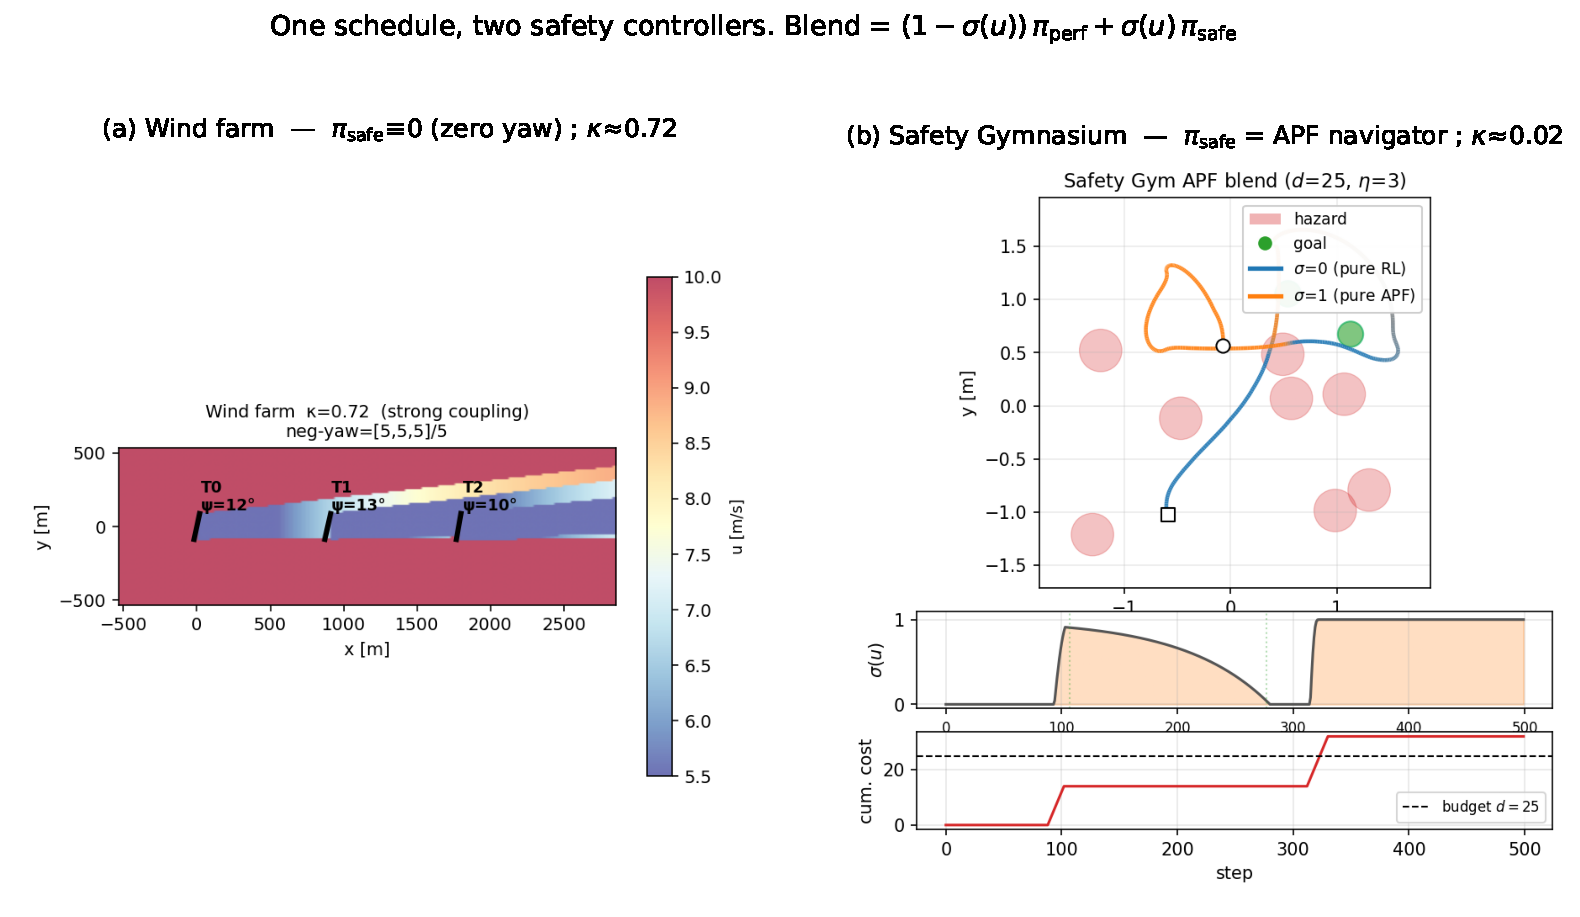
\includegraphics[width=\linewidth]{figures/fig1_blend_overview.pdf}
    \caption{Two domains where pre-trained controllers must be composed under a cumulative budget. (a)~Wind farm: an RL yaw-control policy $\pi_{\mathrm{perf}}$ is blended with a yaw-setpoint $\pi_{\mathrm{safe}}$ (Jensen wake field shown). (b)~Safety Gymnasium PointGoal1: $\pi_{\mathrm{perf}}$ blended with an artificial-potential-field navigator; trajectory colour-coded by blend weight $\sigma(u)$. The linear blend $a = (1-\sigma)\pi_{\mathrm{perf}} + \sigma\pi_{\mathrm{safe}}$ paced by an urgency schedule is the standard inference-time approach. We show it has a fundamental failure mode---the \emph{alignment hazard}---when the two controllers act on opposite sides of a non-convex cost ridge, and propose cost-monotone fixes (\Cref{sec:fixes}, \Cref{fig:alignment_hazard}).}
    \label{fig:setup_overview}
\end{figure}

\textbf{Contributions.}
(1)~We identify the \textbf{alignment hazard}: linear blending of pre-trained controllers under budget pacing is not cost-monotone in $\sigma$ when controllers act on opposite sides of a non-convex cost ridge (\Cref{sec:hazard}).
(2)~A \emph{sufficient condition} for monotonicity (cost convex on the segment $\pi_{\mathrm{perf}}\!\to\!\pi_{\mathrm{safe}}$) with a clean minimal counterexample (\Cref{sec:monotone_theory}).
(3)~Two cost-monotone fixes---\textbf{rejection blending} and \textbf{argmin selection}---built on a single per-step cost probe, both provably no-worse-than-$\pi_{\mathrm{perf}}$ (\Cref{sec:fixes}).
(4)~Empirical demonstration in two domains: wind-farm yaw control with a physics-grounded blade-flap DEL surrogate (direct $\sigma$-sweep, \Cref{sec:sigma_sweep_exp}), and Safety Gymnasium 2D navigation (\Cref{sec:sg_exp}).
(5)~A cross-layout ablation showing the obvious alternative (retrain with a DEL-aware reward) is not a universal substitute: $\beta=1$ direct reward shaping gives Pareto-improving behaviour on one layout and a load/power trade-off on another, so inference-time pacing remains required when retraining for every constraint is infeasible.

\textbf{Deployment claim.}
The method drops into systems that already have an RL performance policy, a domain-specific safety controller, and a damage estimator---none of which are retrained.
The schedule decides when to pace toward the safety controller as budget pressure builds.
We \emph{do not} claim hard budget enforcement: APF on Safety Gym is reactive and can still incur cost (App.~\ref{app:auxiliary}); true enforcement requires a backup invariant such as $C_t + B_{\mathrm{safe}}(t)\!\le\!d$ where $B_{\mathrm{safe}}$ upper-bounds future $\pi_{\mathrm{safe}}$ cost, which we leave to future work.

%----------------------------------------------------------------------
\section{Background}
\label{sec:background}
%----------------------------------------------------------------------

\textbf{Constraint type.}
Long-horizon load and lifetime-fatigue budgets are most accurately modelled as \emph{anytime constraints}~\citep{mcmahan2024anytime}: the cumulative cost may not exceed the budget at any time, almost surely.
\citet{mcmahan2024anytime} show that anytime-feasible Markovian policies are insufficient in general; the state must be augmented with the accumulated cost.
This is also the augmentation SAUTE~\citep{sootla2022saute} uses ($\rho_t$ = remaining budget fraction) for retraining-time pacing.
We adopt the expected-cost CMDP relaxation~\citep{altman1999constrained, ray2019safetygym} as a tractable surrogate, because tractable post-hoc methods are mainly available for the relaxation; the gated fixes we propose (\S\ref{sec:fixes}) guarantee no-worse-than-$\pi_{\mathrm{perf}}$ cost monotonicity, not anytime feasibility.
Closing this gap (e.g., via a backup invariant $C_t + B_{\mathrm{safe}}(t)\!\le\!d$ where $B_{\mathrm{safe}}$ upper-bounds future $\pi_{\mathrm{safe}}$ cost) is future work.

\textbf{Constrained MDPs and Lagrangian methods.}
A CMDP~\citep{altman1999constrained} adds cost-return constraints to the MDP objective: $\max_\pi \mathbb{E}_\pi[\sum_t r_t]$ subject to $\mathbb{E}_\pi[\sum_t c_t] \leq d$~\citep{ray2019safetygym, achiam2017cpo}.
SAC-Lagrangian~\citep{stooke2020responsive} learns a dual variable $\mu$ during training; PID-Lag and CPO~\citep{achiam2017cpo} add stability tweaks.
None of these are post-hoc: changing $d$ requires a new policy.

\textbf{Marginal value of stored resource.}
The urgency-ratio schedule we use is a heuristic stand-in for the dual price on a cumulative constraint.
The same structure appears in reservoir/hydropower operation~\citep{tilmant2008water, you2008hedging} under names like ``water value'' or ``marginal value of stored resource'': release water until the current marginal return equals the marginal expected future loss from depletion; the constraint binds rarely because storage capacity is typically slack, and the dual price is the controlling state.
We make no optimality claim; the schedule is one monotone candidate among many (\S\ref{sec:theory}).

\textbf{Post-hoc composition.}
Energy composition~\citep{urain2023composable, gladstone2025ebt}, classifier guidance~\citep{zhang2025constrained}, control-barrier functions~\citep{xiao2023safediffuser}, and input-convex corrections~\citep{durkin2025picnn} modify pre-trained policies at inference for \emph{instantaneous} constraints.
We extend this tradition to \emph{cumulative} budgets via a time-varying weight, and show the natural linear-blend extension has a sharp failure mode (\S\ref{sec:hazard}).

\textbf{Multi-objective scalarisation.}
A fixed $\alpha P - (1-\alpha)D$ trade-off is memoryless.
Our schedule turns $\alpha$ into a time-varying weight that paces against the realised damage trajectory.

%----------------------------------------------------------------------
\section{Urgency-Ratio Schedule}
\label{sec:theory}
%----------------------------------------------------------------------

\textbf{State-variable identification.}
The natural state for any post-hoc budget-pacing scheduler is the urgency ratio $u=\rho/\tau$.
A toy budget-rate balance under an idealised Boltzmann response $P(\mathrm{risky}\mid\lambda)=P_0\exp(-\alpha\lambda)$ recovers a multiplicative weight $w^*(u) = 1/u$ relative to the time-weighted-average baseline (Appendix~\ref{app:proof}); we treat this as motivation, not derivation.
The Boltzmann assumption is strong, real policies do not respond linearly in log-probability to scalar penalties, and the same state variable $u$ was already identified by SAUTE~\citep{sootla2022saute} as a state-augmentation feature for budget-aware retraining.
What we retain is the observation that any monotone-decreasing $\sigma:[0,\infty)\!\to\![0,1]$ in $u$ is a candidate post-hoc schedule.

\textbf{Practical schedule.}
We use the parametric family
$w(u)=\exp(\eta(1/u-1))$ with $\eta\!\ge\!0$, clamped at $\lambda_{\max}\!=\!10^6$ (Appendix~Fig.~\ref{fig:approx}).
For the two-controller blend (defined in \cref{sec:blend}, Eq.~\ref{eq:blend2}) we map $w(u)$ to a bounded $\sigma\in[0,1]$:
\begin{equation}
    \sigma(u) = \begin{cases}
        0 & u \ge 1, \\
        1 - \exp(-\eta(1/u - 1)) & u < 1.
    \end{cases}
\label{eq:sigma}
\end{equation}
On pace ($u\!\ge\!1$): pure performance policy. Deficit ($u\!<\!1$): smooth ramp toward pure safety controller, sharpness $\eta$.
A hard-wall backstop drives $\sigma\!\to\!1$ for $u\!<\!0.05$.

%----------------------------------------------------------------------
\section{Method}
\label{sec:method}
%----------------------------------------------------------------------

The method has three independent components:
\textbf{(i)}~the schedule $\sigma(u)$ (\emph{how much} safety);
\textbf{(ii)}~the performance policy $\pi_{\mathrm{perf}}$ (what we deploy on pace);
\textbf{(iii)}~the safety controller $\pi_{\mathrm{safe}}$ (what we revert to in deficit).

\subsection{Two-Controller Blend (primary formulation)}
\label{sec:blend}
\begin{equation}
    a_t = (1-\sigma(u_t))\,\pi_{\mathrm{perf}}(s_t) + \sigma(u_t)\,\pi_{\mathrm{safe}}(s_t) .
\label{eq:blend2}
\end{equation}

\textbf{Wind-farm instantiation.}
$\pi_{\mathrm{perf}}$ is an Energy-Based Transformer (EBT) actor trained unconstrained with SAC for 100k steps.
$\pi_{\mathrm{safe}}\!\equiv\!0$ is a zero-yaw setpoint, minimising our per-turbine fatigue surrogate $c=(|y|/\bar{y})^p(v/v_{\mathrm{ref}})^q$ ($p\!=\!2$, $q\!=\!3$).
In production, $\pi_{\mathrm{safe}}$ would be a WakeAdapt-style~\citep{siemensWakeAdapt} setpoint table minimising farm-level DEL.

\textbf{Safety Gymnasium instantiation.}
$\pi_{\mathrm{perf}}$ is a SAC/MLP actor trained unconstrained for 200k steps.
$\pi_{\mathrm{safe}}$ is an artificial-potential-field navigator: $F_{\mathrm{goal}}=\mathrm{norm}(g-x)$ + $F_{\mathrm{rep}}=k_r\sum_i (x-h_i)/\|x-h_i\|^3$, mapped to body-frame $(\mathrm{thrust},\mathrm{turn})$.
No learning; uses only the hazard/goal geometry that every CBF-based safe-RL method assumes access to.

\subsection{Gradient-Correction Variant}
\label{sec:gradient}
When an action-dependent cost $\nabla_a c$ or $\nabla_a Q_c$ is available, a single gradient step replaces the explicit $\pi_{\mathrm{safe}}$:
\begin{equation}
    a_t \leftarrow \pi_{\mathrm{perf}}(s_t) - \lambda_{\mathrm{gs}}\cdot w(u_t)\cdot \alpha_{\mathrm{g}}\cdot \nabla_a c(s_t, a_t),
\label{eq:gradient_correction}
\end{equation}
iterated $K$ steps. This is Eq.~\ref{eq:blend2} with $\pi_{\mathrm{safe}}(s)\!\approx\!\pi_{\mathrm{perf}}(s) - \alpha_{\mathrm{g}}\nabla_a c$ implicitly defined.

\subsection{Coupling Strength \texorpdfstring{$\kappa$}{kappa}: Which Variant?}
\label{sec:scope}

The gradient variant requires a non-trivial $\nabla_a Q_c$.
We quantify this by
\begin{equation}
    \kappa := \mathbb{E}_{(s,a)\sim\pi}\|\nabla_a Q_c(s,a)\|_2 \,\big/\, \mathbb{E}_{(s,a)\sim\pi}\|\nabla_s Q_c(s,a)\|_2,
\label{eq:kappa}
\end{equation}
measured on logged rollouts.
Large $\kappa$: gradient correction suffices.
Small $\kappa$: action-gradient is weak; explicit $\pi_{\mathrm{safe}}$ is required.

\begin{table}[h]
\centering
\caption{Coupling strength $\kappa$ per domain (2000 on-policy samples). Large $\kappa$: gradient correction suffices. Small $\kappa$: explicit $\pi_{\mathrm{safe}}$ blend required.}
\label{tab:coupling}
\begin{tabular}{lcccl}
\toprule
Domain & $\mathbb{E}\|\nabla_a Q_c\|$ & $\mathbb{E}\|\nabla_s Q_c\|$ & $\kappa$ & Recommended variant \\
\midrule
Wind farm (3-turb)     & $0.69\!\pm\!0.34$ & $0.97\!\pm\!0.26$ & $\mathbf{0.72}$ & gradient correction (Eq.~\ref{eq:gradient_correction}) \\
Safety Gym (PointGoal) & $0.99\!\pm\!0.69$ & $49.8\!\pm\!12.5$ & $\mathbf{0.02}$ & explicit $\pi_{\mathrm{safe}}$ blend (Eq.~\ref{eq:blend2}) \\
\bottomrule
\end{tabular}
\end{table}

\begin{algorithm}[t]
\caption{Urgency-Ratio Controller Blending (with safeguards)}
\label{alg:budget}
\begin{algorithmic}[1]
\REQUIRE Performance policy $\pi_{\mathrm{perf}}$, safety controller $\pi_{\mathrm{safe}}$, budget $d>0$, horizon $T$, sharpness $\eta$, hard-wall threshold $u_{\mathrm{hw}}\!=\!0.05$, action bounds $[a_{\min}, a_{\max}]$
\STATE $C_0 \gets 0$
\FOR{$t = 0, 1, \ldots, T-1$}
    \STATE $\rho_t \gets \max((d - C_t)/d,\, 0)$;\quad $\tau_t \gets \max((T-t)/T,\, 1/T)$
    \IF{$\rho_t = 0$ \textbf{or} $\tau_t \le 1/T$}
        \STATE $\sigma_t \gets 1$ \COMMENT{budget exhausted or last step: $\pi_{\mathrm{safe}}$ takes over}
    \ELSE
        \STATE $u_t \gets \rho_t / \tau_t$
        \STATE $\sigma_t \gets 0$ if $u_t \ge 1$ else $1 - \exp(-\eta(1/u_t - 1))$
        \STATE \textbf{if} $u_t < u_{\mathrm{hw}}$ \textbf{then} $\sigma_t \gets 1$ \COMMENT{hard-wall backstop}
    \ENDIF
    \STATE $a_t \gets \mathrm{clip}((1-\sigma_t)\,\pi_{\mathrm{perf}}(s_t) + \sigma_t\,\pi_{\mathrm{safe}}(s_t),\; a_{\min},\, a_{\max})$
    \STATE Execute $a_t$; observe $c_t$; $C_{t+1} \gets C_t + c_t$
\ENDFOR
\end{algorithmic}
\end{algorithm}

%----------------------------------------------------------------------
\section{The Alignment Hazard}
\label{sec:hazard}
%----------------------------------------------------------------------

The two-controller blend (\ref{eq:blend2}) implicitly assumes that as $\sigma$ moves from $0$ to $1$, cumulative cost $C[a(\sigma)]$ moves monotonically from $C[\pi_{\mathrm{perf}}]$ to $C[\pi_{\mathrm{safe}}]$.
We show this assumption can fail strictly: the linear midpoint $a(\sigma)$ can have cost higher than both endpoints.
We call this the \textbf{alignment hazard}.

\subsection{A Minimal Counterexample}
\label{sec:counterexample}

Consider a one-step setting with scalar action $a \in \mathbb{R}$, constant controllers $\pi_{\mathrm{perf}} \equiv -1$ and $\pi_{\mathrm{safe}} \equiv +1$, and cost
\begin{equation}
    c(a) = \exp\!\big(-a^2\big),
\label{eq:counterexample_cost}
\end{equation}
modelling a load whose peak is at the neutral action.
Then $a(\sigma) = -1 + 2\sigma$, so $C[a(0)] = C[a(1)] = e^{-1} \approx 0.37$, while $C[a(0.5)] = c(0) = 1$.
The linear blend at $\sigma=0.5$ has $\sim2.7\times$ the cost of either endpoint.

\textbf{This is not just Jensen's inequality.}
That a non-convex function's midpoint can exceed its endpoints is elementary in the abstract.
Our contribution is twofold.
First, we identify that the \emph{composition literature}---energy composition~\citep{urain2023composable}, classifier guidance~\citep{zhang2025constrained}, control-barrier-function shields~\citep{xiao2023safediffuser}, input-convex corrections~\citep{durkin2025picnn}, and the budget-paced blends we just defined---implicitly assumes the segment-convexity condition without checking it.
Second, we show the failure is generic on directional action manifolds.

\textbf{Where this happens in practice.}
Any action that is a \emph{direction} or \emph{angle} (yaw setpoint, attack heading, steering angle, satellite pointing, gait phase) and any cost with a ``ridge'' interior to the operating range exposes this hazard.
Wind-turbine blade-flap damage equivalent load (DEL) is exactly this case, with a detail that matters: probing our DLC12 surrogate directly (\cref{fig:del_ridge}) shows the flap-DEL ridge is \emph{not} at $0^\circ$ but at $-9^\circ$ to $-14^\circ$ for freestream and moderately waked inflow---consistent with the known yaw-asymmetry of flap loads that motivates positive-yaw wake steering in practice.
When $\pi_{\mathrm{perf}}$ yaws negative of the ridge (e.g., $-15^\circ$) and $\pi_{\mathrm{safe}}$ yaws positive (e.g., $+7.5^\circ$), the linear blend at intermediate $\sigma$ crosses the ridge.

\begin{figure}[h]
\centering
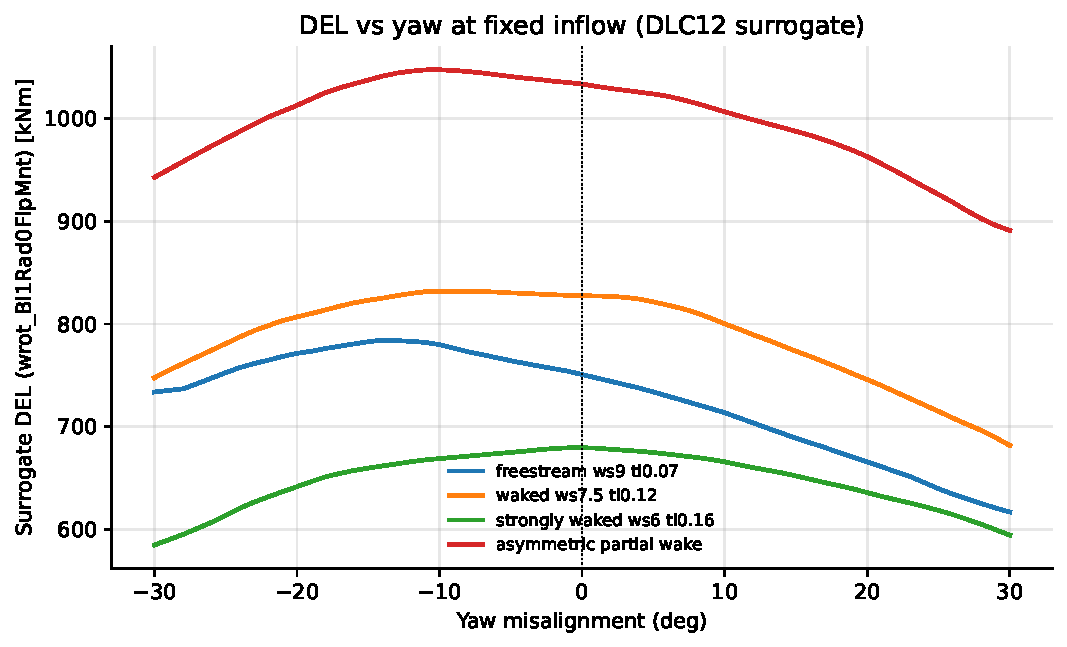
\includegraphics[width=0.7\linewidth]{figures/del_ridge_probe.pdf}
\caption{The cost ridge, measured. DLC12 surrogate flap DEL vs yaw at four fixed inflow conditions. The ridge peaks at $-14^\circ$ (freestream), $-9^\circ$ (waked), $0^\circ$ (strongly waked), $-10^\circ$ (asymmetric partial wake)---\emph{not} at the neutral direction except under strong waking. This measured ridge location explains the $\sigma$-sweep peak position in \cref{fig:sigma_sweep} (peak at $\sigma=0.4$, mean yaw $\approx-8^\circ$): the blend's DEL maximum occurs where the trajectory crosses the actual ridge, exactly as the segment-convexity analysis predicts.}
\label{fig:del_ridge}
\end{figure}

\subsection{Cost-Monotonicity: A Sufficient Condition}
\label{sec:monotone_theory}

\textbf{Proposition (cost-convex segment is monotone).}
Let $A(s,\sigma) = (1-\sigma)\pi_{\mathrm{perf}}(s) + \sigma\pi_{\mathrm{safe}}(s)$.
If for every state $s$ the cost $c(s,\cdot)$ is convex on the segment $\{A(s,\sigma): \sigma\in[0,1]\}$, then the per-step cost $c(s, A(s,\sigma))$ is convex in $\sigma$, hence bounded above by $\max\{c(s, \pi_{\mathrm{perf}}), c(s, \pi_{\mathrm{safe}})\}$.
Under fixed visited-state distribution (one-step or open-loop), the cumulative cost $C[a(\sigma)]$ is convex in $\sigma$.

\emph{Proof.} Convex composition with affine map; expectation preserves convexity. $\square$

The hazard arises precisely when the segment-convexity assumption \emph{fails}, which is the typical case on directional manifolds.

\subsection{Cost-Monotone Fixes}
\label{sec:fixes}

We propose two replacements for the linear blend, both relying on a single per-step cost probe and \emph{provably no-worse-than}-$\pi_{\mathrm{perf}}$.

\paragraph{Rejection blend (B3).}
At each step, form the candidate blended action $a_{\mathrm{blend}} = (1-\sigma(u))\pi_{\mathrm{perf}}(s) + \sigma(u)\pi_{\mathrm{safe}}(s)$ and probe \emph{the blended action itself}: evaluate $\hat c_{\mathrm{blend}} = c(s, a_{\mathrm{blend}})$ and $\hat c_{\mathrm{perf}} = c(s, \pi_{\mathrm{perf}}(s))$ via a one-step cost surrogate, then
\begin{equation}
    a_{\mathrm{eff}}(s,u) =
    \begin{cases}
        a_{\mathrm{blend}} & \hat c_{\mathrm{blend}} \le \hat c_{\mathrm{perf}}, \\
        \pi_{\mathrm{perf}}(s) & \text{otherwise.}
    \end{cases}
\label{eq:rejection}
\end{equation}
The probe is computed per state (per turbine in the multi-agent setting).
\emph{Probing the blended action, not the endpoints, is essential}: an endpoint comparison ($\hat c_{\mathrm{safe}}$ vs $\hat c_{\mathrm{perf}}$) can certify a cheap safe endpoint while the executed intermediate action sits on the cost ridge---the very failure this paper analyses.
We verify this distinction empirically: at the zero-crossing hazard regime, the endpoint-probing variant produces cumulative DEL statistically indistinguishable from the unguarded linear blend ($63416$ vs $63420$), while the blended-action probe avoids the ridge ($62847$; \cref{tab:fix_recovery_zero}).
The theoretical gap is not hypothetical---it costs exactly the hazard the gate was meant to prevent.

\paragraph{Argmin selection (B1).}
A harder variant collapses to a binary choice between the endpoints: execute $\pi_{\mathrm{safe}}$ if $\hat c_{\mathrm{safe}} < \hat c_{\mathrm{perf}}$, else $\pi_{\mathrm{perf}}$.
This sacrifices the smooth schedule but never executes an intermediate action, eliminating ridge crossings entirely.

\textbf{Cost monotonicity.}
For both fixes, $c(s, a_{\mathrm{eff}}) \le c(s, \pi_{\mathrm{perf}}(s))$ per state---rejection by the explicit probe of the executed action, argmin by minimisation over the two endpoints---so the cumulative cost satisfies $C[a_{\mathrm{eff}}] \le C[\pi_{\mathrm{perf}}]$ under a fixed visited-state distribution and an accurate probe.
Both caveats are real: in closed loop the state distribution shifts with the executed actions, and probe error transfers linearly into the guarantee.
Linear blend has no guarantee of any kind.

\textbf{Cost of the probe.}
For surrogate-based costs (e.g., our load surrogate), the probe is one extra surrogate forward pass per candidate per step.
For learned critics ($Q_c$), it is one extra critic call.
Both are cheap relative to policy inference and step simulation.

%----------------------------------------------------------------------
\section{Experiments}
\label{sec:results}
%----------------------------------------------------------------------

\textbf{Setup.}
We train three EBT-SAC actors to expose the hazard regime:
(i)~$\pi_{\mathrm{perf}}^{\mathrm{MM,DEL}}$ on the multi\_modal 3-turbine layout with a DEL-aware reward $r' = r - \beta \sum_i \mathrm{DEL}_i / \mathrm{DEL}_{\mathrm{ref}}$ at $\beta=1$;
(ii)~$\pi_{\mathrm{perf}}^{\mathrm{MM,std}}$ on the same layout with the standard reward (no DEL penalty);
(iii)~$\pi_{\mathrm{perf}}^{\mathrm{stag4,DEL}}$ on the stag4\_5d 4-turbine layout with DEL-aware reward at $\beta=1$.
All actors trained 200k steps on WindGym with the PyWake backend.
$\pi_{\mathrm{safe}}$ is a yaw setpoint controller: a P-controller driving each turbine toward a target $y^{\mathrm{tgt}}$ at the actuator rate.
DEL is scored per-step by a DLC12 sector-averaged ANN load surrogate~\citep{guillore2024sectoravg} evaluated on the realised flow and yaw.
Cumulative quantities are summed over 200-step rollouts; episode counts per configuration are stated with each result.
Power is reported in GW-step (the sum of farm power over the 200 steps; divide by 200 for the farm-average in GW), and DEL in kNm cumulative.

\subsection{The Direct Test: Cost vs \texorpdfstring{$\sigma$}{sigma} at Fixed Controllers}
\label{sec:sigma_sweep_exp}

The Proposition of \cref{sec:monotone_theory} concerns non-monotonicity of $C[a(\sigma)]$ in $\sigma$ at fixed $\pi_{\mathrm{perf}}, \pi_{\mathrm{safe}}$, so the matching experiment fixes both controllers and sweeps $\sigma$.
We fix $\pi_{\mathrm{perf}}$ (the DEL-aware MM actor, settling at $\bar y \approx -15^\circ$) and sweep $\sigma\in\{0, 0.1, \ldots, 1.0\}$ for three choices of $\pi_{\mathrm{safe}}$:
a hazardous configuration ($y^{\mathrm{tgt}}=+7.5^\circ$, where the segment $\pi_{\mathrm{perf}}\!\to\!\pi_{\mathrm{safe}}$ crosses the zero-yaw DEL ridge and both endpoints have low DEL), a co-directional control ($y^{\mathrm{tgt}}=-25^\circ$, segment stays on one side of the ridge), and a high-DEL-endpoint variant ($y^{\mathrm{tgt}}=+15^\circ$).

\Cref{fig:sigma_sweep} shows the result.
In the hazardous configuration ($n=50$ episodes per $\sigma$), cumulative DEL peaks at $\sigma=0.4$ ($63264$), strictly above the $\sigma\!=\!0$ endpoint ($63052$) by $+212$ ($3\sigma$ of the standard error) and above the $\sigma\!=\!1$ endpoint ($62681$) by $+583$ ($8\sigma$).
Two points guard the statistics.
First, the peak location is not post-hoc: the blend trajectory's mean yaw at $\sigma=0.4$ is $\approx-8^\circ$, which coincides with the surrogate's independently measured DEL ridge at $-9^\circ$ for waked inflow (\cref{fig:del_ridge})---the peak is where the mechanism puts it.
Second, even treating the peak as selected from the 11 sweep points, a Bonferroni correction leaves the $\sigma\!=\!0$ separation significant ($p \approx 0.003 \times 11 \approx 0.03$) and the $\sigma\!=\!1$ separation untouched.
\emph{This is the alignment hazard, demonstrated on the axis the theory speaks to: the linear blend is anti-Pareto in $\sigma$.}
The co-directional control is monotone in $\sigma$, as the segment-convexity condition predicts.

\begin{figure}[h]
\centering
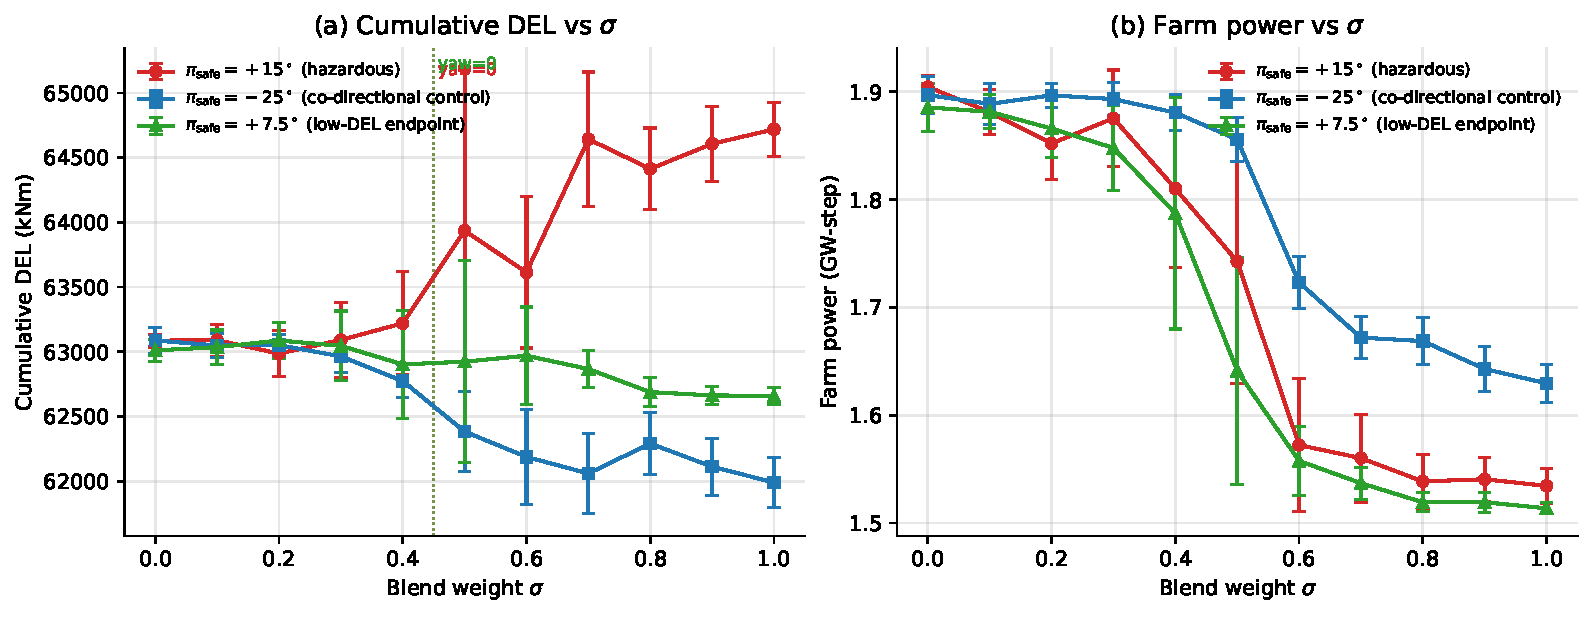
\includegraphics[width=0.95\linewidth]{figures/sigma_sweep.pdf}
\caption{Cumulative DEL and farm power vs blend weight $\sigma$ at fixed $\pi_{\mathrm{perf}}$ (DEL-aware MM actor, settling at $\bar y \approx -15^\circ$) and three $\pi_{\mathrm{safe}}$ choices; error bars are standard error of the mean.
\textbf{Red ($\pi_{\mathrm{safe}}=+7.5^\circ$, hazardous, $n=50$):} both endpoints are low-DEL ($63052$ at $\sigma\!=\!0$, $62681$ at $\sigma\!=\!1$); the segment passes through the zero-yaw ridge.
A clear hump appears at $\sigma\!=\!0.4$, DEL $=63264$ (peak yaw $\approx -8^\circ$, in the transition toward zero), strictly above the $\sigma\!=\!0$ endpoint by $+212$ (3$\sigma$) and above the $\sigma\!=\!1$ endpoint by $+583$ (8$\sigma$).
This is the experiment that directly matches the Proposition (\cref{sec:monotone_theory}).
\textbf{Blue ($\pi_{\mathrm{safe}}=-25^\circ$, co-directional control, $n=10$):} DEL is monotone in $\sigma$, consistent with the segment staying on one side of the cost ridge.
\textbf{Green ($\pi_{\mathrm{safe}}=+15^\circ$, high-DEL endpoint, $n=50$):} DEL increases monotonically because $\pi_{\mathrm{safe}}$ at $+15^\circ$ is itself a higher-DEL setpoint than $\pi_{\mathrm{perf}}$; the strict-above-both regime is not reached here, but a local non-monotonicity at the yaw=0 crossing is consistent with the predicted ridge.}
\label{fig:sigma_sweep}
\end{figure}

\subsection{The Panoramic View: Sweeping \texorpdfstring{$\pi_{\mathrm{safe}}$}{pi-safe} Direction at Fixed \texorpdfstring{$\sigma$}{sigma}}
\label{sec:hazard_wf}

A complementary view fixes $\sigma=0.7$ and sweeps the $\pi_{\mathrm{safe}}$ target across $\{-25^\circ, \ldots, +25^\circ\}$: each grid point is a different deployment configuration an operator might choose.
\Cref{tab:linear_hazard_mm} shows the linear blend at $y^{\mathrm{tgt}}=0$ drives mean yaw to $\approx 0^\circ$ where blade-flap DEL is locally maximal: total DEL ($63375$) exceeds both immediate neighbours by $\approx 0.7\%$, and farm power is locally depressed ($-10\%$ vs the higher-power neighbour).
A separate, larger effect appears at $y^{\mathrm{tgt}}=+25^\circ$ from saturated wake misalignment (a different mechanism; see \cref{sec:fix_exp}).
\Cref{fig:alignment_hazard}a plots the same sweep in the power-DEL plane, with the gated fixes overlaid.

\begin{table}[h]
\centering
\caption{Linear blend at $\sigma=0.7$ on multi\_modal (DEL-aware actor), $n=10$. The row at $y^{\mathrm{tgt}}=0$ is the zero-crossing regime: blend yaw $\approx 0^\circ$ is the local DEL maximum.}
\label{tab:linear_hazard_mm}
\small
\begin{tabular}{rrrrrr}
\toprule
$y^{\mathrm{tgt}}$ & Power (GW-step) & DEL\textsubscript{T0} & DEL\textsubscript{T1} & DEL\textsubscript{T2} & DEL\textsubscript{tot} \\
\midrule
$-25^\circ$ & 1.69 & 20701 & 20748 & 20853 & 62302 \\
$-15^\circ$ & 1.83 & 20888 & 20770 & 20816 & 62474 \\
$-7.5^\circ$ & 1.79 & 20984 & 20973 & 20956 & 62913 \\
$\mathbf{0^\circ}$ & \textbf{1.61} & \textbf{21132} & \textbf{21132} & \textbf{21111} & \textbf{63375} \\
$+7.5^\circ$ & 1.53 & 20887 & 20934 & 20887 & 62708 \\
$+15^\circ$ & 1.53 & 21366 & 21399 & 21336 & 64101 \\
$+25^\circ$ & 1.50 & 21699 & 21690 & 21640 & 65029 \\
\bottomrule
\end{tabular}
\end{table}

\begin{figure}[h]
\centering
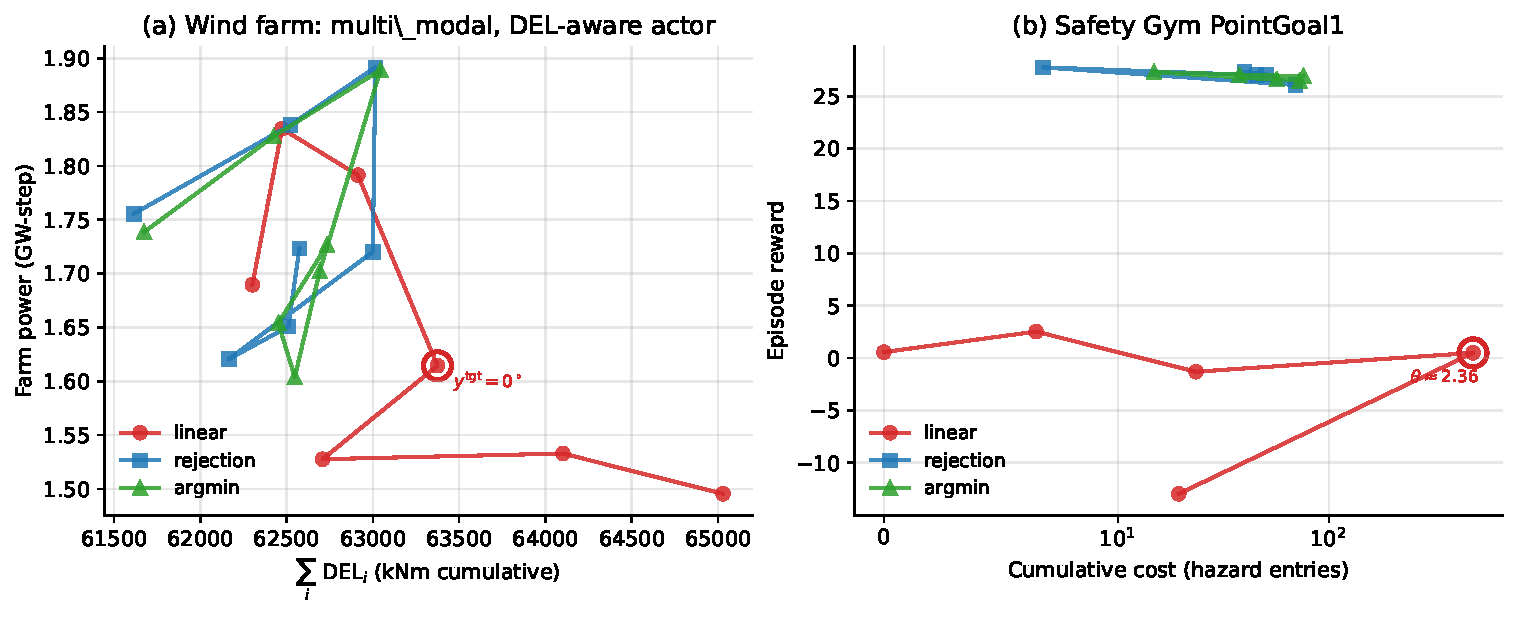
\includegraphics[width=0.92\linewidth]{figures/alignment_hazard.pdf}
\caption{The alignment hazard in the power--cost plane. \textbf{(a)} Wind farm (multi\_modal, DEL-aware actor): farm power vs cumulative DEL across $\sigma=0.7$ linear blend at seven $\pi_{\mathrm{safe}}$ yaw targets $\in[-25^\circ,+25^\circ]$. Linear blend (red) zigzags into an anti-Pareto bulge at $y^{\mathrm{tgt}}=0$ (circled). Rejection (blue) and argmin (green) recover the Pareto frontier. \textbf{(b)} Safety Gymnasium PointGoal1: episode reward vs cumulative cost across APF rotations $\theta\in\{0,\pi/4,\pi/2,3\pi/4,\pi\}$. Linear collapses at $\theta\approx 2.36$ (circled, $C\!=\!483$, $R\!=\!0.5$); rejection and argmin stay near $\pi_{\mathrm{perf}}$'s reward (${\approx}27$) at low cost.}
\label{fig:alignment_hazard}
\end{figure}

\subsection{Gated Fixes Recover the Frontier}
\label{sec:fix_exp}

\textbf{At the zero-crossing regime} ($y^{\mathrm{tgt}}=0$, \cref{tab:fix_recovery_zero}), rejection and argmin drive $\sigma_{\mathrm{eff}}$ away from $0.7$ on turbines where the 1-step probe says blending would worsen DEL: recovered farm power is $+6.2\%$ (rejection) and $+6.2\%$ (argmin) above the linear blend, with DEL reduced.
The same table carries the empirical confirmation of the probe-placement argument from \cref{sec:fixes}: the endpoint-probing variant---which certifies the safe \emph{endpoint} but executes the \emph{intermediate} action---lands on the ridge anyway, with DEL essentially equal to the unguarded linear blend.

\begin{table}[h]
\centering
\caption{Alignment-hazard regime at the zero crossing ($\sigma=0.7$, $y^{\mathrm{tgt}}=0^\circ$, MM DEL-aware actor, $n=10$): linear blend through the DEL ridge vs gated fixes. The endpoint-probing variant fails to avoid the ridge (DEL $\approx$ linear), confirming that the probe must evaluate the executed (blended) action.}
\label{tab:fix_recovery_zero}
\small
\begin{tabular}{lrr}
\toprule
Mode & Power (GW-step) & DEL\textsubscript{tot} \\
\midrule
Linear & 1.62 & 63420 \\
Rejection (blended-action probe) & 1.72 & 62847 \\
Rejection (endpoint probe; flawed) & 1.77 & 63416 \\
Argmin & 1.72 & 62971 \\
\midrule
\multicolumn{1}{l}{\emph{$\Delta$ rejection vs linear:}} & $+6.2\%$ pwr & $-0.9\%$ DEL \\
\multicolumn{1}{l}{\emph{$\Delta$ argmin vs linear:}} & $+6.2\%$ pwr & $-0.7\%$ DEL \\
\bottomrule
\end{tabular}
\end{table}

\textbf{At the saturated-wake regime} ($y^{\mathrm{tgt}}=+25^\circ$), a second, distinct anti-Pareto effect appears: the blend pushes yaw deep into the saturated-wake-misalignment region of the DEL surrogate.
This is a different mechanism from the zero-crossing alignment hazard---wake saturation, not segment-convexity violation at the neutral ridge---but it is also a regime where linear blending hurts and the gated fixes recover, by a much larger margin (\cref{tab:fix_recovery_sat}).
We label it separately; it is not the hazard the paper is named for.

\begin{table}[h]
\centering
\caption{Saturated-wake regime ($\sigma=0.7$, $y^{\mathrm{tgt}}=+25^\circ$, MM DEL-aware actor, $n=10$): a separate large-yaw effect, not the zero-crossing alignment hazard. Rejection uses the corrected blended-action probe.}
\label{tab:fix_recovery_sat}
\small
\begin{tabular}{lrrr}
\toprule
Mode & Power (GW-step) & DEL\textsubscript{tot} & $\sigma_{\mathrm{eff}}$ mean (T0, T1, T2) \\
\midrule
Linear & 1.52 & 64703 & $(0.70, 0.70, 0.70)$ \\
Rejection (blended-action probe) & 1.66 & 62344 & $(0.32, 0.45, 0.40)$ \\
Argmin & 1.65 & 62740 & $(0.25, 0.41, 0.35)$ \\
\midrule
\multicolumn{1}{l}{\emph{$\Delta$ rejection vs linear:}} & $+9.2\%$ pwr & $-3.6\%$ DEL \\
\multicolumn{1}{l}{\emph{$\Delta$ argmin vs linear:}} & $+8.6\%$ pwr & $-3.0\%$ DEL \\
\bottomrule
\end{tabular}
\end{table}

Full linear/rejection/argmin × $y^{\mathrm{tgt}}$ grids for all three actor-layout combinations appear in App.~\ref{app:full_sweep}; on MM (both actors) the linear curve has a clear DEL bulge centred at $y^{\mathrm{tgt}}=0$, and the blended-probe fixes never produce intermediate-yaw bulges.
(Earlier grids in App.~\ref{app:full_sweep} report the endpoint-probing variant under the label ``rejection''; the main-text tables use the corrected blended-action probe.)

\subsection{Second Domain: 2D Navigation}
\label{sec:sg_exp}

We repeat the $\pi_{\mathrm{safe}}$-direction sweep in Safety Gymnasium PointGoal1 with an APF (artificial-potential-field) safety controller rotated by $\theta \in \{0, \pi/4, \pi/2, 3\pi/4, \pi\}$.
\emph{The rotation is a synthetic misalignment probe, not a plausible deployed controller}: it parameterises how far $\pi_{\mathrm{safe}}$'s direction deviates from its design intent, standing in for realistic misalignment sources (a stale goal position, an APF tuned for a different hazard layout, a miscalibrated frame transform) whose direction error we cannot sweep cleanly.
\Cref{tab:sg_hazard} shows the worst-case $\theta=3\pi/4$ regime: linear blend incurs $C=483$ (and $R\approx 0.5$, near-zero goal progress), while rejection cuts cost to $C=50$ and argmin to $C=15$, both retaining reward $R\approx 27$ matching $\pi_{\mathrm{perf}}$ alone.
The hazard exists on directional action manifolds beyond yaw control, and its magnitude here is an order of magnitude larger than in wind: the cost surface around a hazard disk is far sharper than the blade-flap DEL ridge.

\begin{table}[h]
\centering
\caption{Safety-Gym worst-case alignment-hazard regime ($\sigma=0.7$, $\theta=3\pi/4$, PointGoal1, $n=10$ ep): linear blend vs fixes.}
\label{tab:sg_hazard}
\small
\begin{tabular}{lrr}
\toprule
Mode & Reward & Cost \\
\midrule
Linear & $0.50 \pm 2.75$ & $483 \pm 108$ \\
Rejection & $27.08 \pm 1.35$ & $50 \pm 16$ \\
Argmin & $27.30 \pm 0.93$ & $15 \pm 16$ \\
$\pi_{\mathrm{perf}}$ alone (reference) & $27$ & $45$ \\
\bottomrule
\end{tabular}
\end{table}

\subsection{Scoping: Where the Hazard Does Not Appear, and Why Retraining Is Not a Substitute}
\label{sec:scoping}

\textbf{Layout sensitivity.}
On stag4\_5d, $\sigma$-sweeps in three directions ($y^{\mathrm{tgt}} \in \{-15^\circ, 0^\circ, +25^\circ\}$, $n=30$) are all monotone: the DEL surface for this layout is dominated by an overall yaw-tilt trend with no significant local maximum at the neutral direction.
Likewise the direction sweep at fixed $\sigma$ produces a monotone power-vs-DEL trade-off, not a U-shape.
\emph{The hazard requires $\pi_{\mathrm{perf}}$ and $\pi_{\mathrm{safe}}$ to straddle a sufficiently sharp cost ridge}; whether a given layout/wind regime has one is an empirical question the segment-convexity condition turns into a checkable property.

\textbf{Retraining is not a universal substitute.}
The natural objection to inference-time composition is direct reward shaping: train with $r' = r - \beta\sum_i \mathrm{DEL}_i$ and skip blending.
\Cref{tab:cross_layout_actor} shows this is layout-pathological at fixed $\beta$: the DEL-aware actor Pareto-dominates zero-yaw on multi\_modal ($+14\%$ power, $-3\%$ DEL) but trades $+5$--$7\%$ DEL for $+22\%$ power on stag4\_5d, and the standard actor wastes $6\%$ power on multi\_modal.
The sensitivity holds even \emph{within} a single layout: sweeping $\beta\in\{0.5, 1, 2\}$ on multi\_modal, only $\beta=1$ Pareto-dominates zero-yaw---at $\beta=0.5$ the downstream turbine's DEL exceeds the zero-yaw baseline by $+5.0\%$ ($+1046$ kNm), and at $\beta=2$ by $+1.0\%$ ($+204$ kNm), despite both retaining a $16$--$18\%$ power advantage ($n=10$ episodes each).
$\beta$ must be chosen per layout \emph{and per value}; without retraining for every constraint, the operator needs deployment-time composition---and then must avoid the hazard.

\begin{table}[h]
\centering
\caption{Actor vs zero-yaw baseline across layouts ($n=10$ episodes, 200 steps).}
\label{tab:cross_layout_actor}
\small
\begin{tabular}{llrrr}
\toprule
Layout & Actor & $\Delta$ Power & $\Delta$ DEL/turb & Pareto vs zero? \\
\midrule
multi\_modal & DEL-aware $\beta\!=\!1$ & $+14\%$ & $[-3.2\%, -5.1\%, -0.7\%]$ & both axes \\
multi\_modal & Standard (no DEL) & $-6\%$ & $[-2.0\%, -2.4\%, -2.7\%]$ & DEL only \\
stag4\_5d & DEL-aware $\beta\!=\!1$ & $+22\%$ & $[+7.0\%, +4.5\%, +5.0\%, +4.3\%]$ & power only \\
\bottomrule
\end{tabular}
\end{table}

\textbf{Auxiliary linear-blend validation.}
We additionally validate budget tracking under the original (pre-hazard-discovery) linear-blend framework in two settings where the safe controller is co-directional with $\pi_{\mathrm{perf}}$ and the hazard does not arise: zero-yaw safety on wind farm and an artificial-potential-field navigator on Safety Gymnasium.
Linear blend tracks per-turbine DEL budgets within tolerance on the wind farm, and gives a reward-favourable operating point versus SAC-Lagrangian and SAUTE retraining baselines on Safety Gymnasium.
Full tables, including retraining-baseline comparisons, are reported in \Cref{app:auxiliary}.

%----------------------------------------------------------------------
\section{Related Work}
\label{sec:related}
%----------------------------------------------------------------------

\textbf{Anytime-constrained RL.}
\citet{mcmahan2024anytime} formalise constraints that must hold at every step almost surely (not just in expectation); they prove Markovian policies are insufficient and propose augmenting state with cumulative cost.
The urgency-ratio variable $\rho_t = (d-C_t)/d$ is exactly such an augmentation.
We adopt the expected-cost relaxation as a tractable surrogate; our gated fixes provide cost-monotonicity, not anytime feasibility.

\textbf{Constrained MDPs.}
Lagrangian methods~\citep{altman1999constrained, achiam2017cpo, stooke2020responsive, chen2025predictive} learn dual variables during training.
SAUTE~\citep{sootla2022saute} augments state with $\rho_t$ but retrains per budget; we run it as a baseline (App.~\ref{app:auxiliary}).
TREBI~\citep{lin2023trebi} handles real-time budget changes via diffusion-specific training.
We freeze both controllers and use a closed-form $\sigma(u)$ at inference, with a gated composition that survives the alignment hazard.

\textbf{Marginal value of stored resource.}
Reservoir and hydropower operation~\citep{tilmant2008water, you2008hedging} computes the marginal value of remaining storage via stochastic dynamic programming (``water value'').
The urgency-ratio schedule is a closed-form heuristic in the same spirit.
The decades-old structure---slack most of the time, binding rarely---is exactly the long-horizon DEL-budget setting.

\textbf{Post-hoc composition.}
Energy composition~\citep{urain2023composable}, classifier guidance~\citep{zhang2025constrained}, CBFs~\citep{xiao2023safediffuser}, and input-convex corrections~\citep{durkin2025picnn} handle instantaneous constraints.
Blending with an explicit safety controller is long-standing in robotics (reactive hierarchies, shielding, override layers).
\emph{All of these implicitly assume the segment-convexity condition of \Cref{sec:monotone_theory}}; our finding is that this assumption can fail sharply on directional action manifolds, and that gated composition is a cheap fix.

\textbf{Budget pacing.}
Budget allocation in advertising~\citep{balseiro2023budget} and bandits with knapsacks~\citep{agrawal2014bandits} share the allocation-across-time structure.
We adopt the urgency-ratio framework from optimal execution~\citep{almgren2001optimal}.

\textbf{Load-constrained wake steering with RL.}
\citet{multiobj2026loadwake} train independent SAC actors with sector-averaged DEL surrogates on WindGym and shaped reward $r' = r - \beta\,\mathbf{1}[\Delta\mathrm{DEL} > \tau]$; FALCON~\citep{falcon2021} treats wake steering as a power-vs-lifetime Pareto problem via multi-agent DRL; WFCRL~\citep{wfcrl2025} provides a MARL benchmark with fatigue cost.
These works adopt \emph{expected-cost / reward-shaping} formulations.
Our contribution is orthogonal: we argue the constraint is more naturally anytime, and we expose a composition hazard that none of these works note.
WakeAdapt~\citep{siemensWakeAdapt} is the closest industrial $\pi_{\mathrm{safe}}$ analogue.

\textbf{Coupling-strength scope.}
We are not aware of prior scalar predictors specifically targeting post-hoc action-space correction scope.
$\kappa$ is the gradient \emph{ratio} between state and action, usable as an a-priori diagnostic on logged data.

%----------------------------------------------------------------------
\section{Discussion}
\label{sec:discussion}
%----------------------------------------------------------------------

\textbf{What the alignment hazard means for policy composition.}
The hazard is a sharp failure mode of inference-time policy composition, not a wind-specific quirk.
Any setting in which the action lives on a directional manifold (yaw, steering, heading, satellite pointing, gait phase) and the cost is non-convex along the segment $\pi_{\mathrm{perf}}\!\to\!\pi_{\mathrm{safe}}$ is exposed.
The composition literature implicitly assumes the segment-convex condition of \Cref{sec:monotone_theory} without checking it.
Our two-domain demonstration shows the failure is severe on 2D navigation ($-97\%$ goal reward at the worst-case rotation, midpoint cost strictly above both endpoints) and statistically robust in wind ($n=50$ $\sigma$-sweep at a low-DEL $\pi_{\mathrm{safe}}$: midpoint DEL exceeds both endpoints by $+212$ and $+583$ kNm, $3\sigma$ and $8\sigma$ respectively; \Cref{fig:sigma_sweep}). The magnitude is larger in 2D navigation; the wind effect is smaller in absolute terms but unambiguous after noise reduction. The cost-monotone fixes recover the Pareto frontier with one extra cost probe per step.

\textbf{Two flavours of long-horizon budget.}
The two domains expose complementary regimes.
On the wind farm at fixed wind direction, the DEL budget is slack on any single episode---zero yaw alone is power-competitive with the unconstrained actor, so the only task is avoiding the hazard, not preserving a large RL advantage.
On Safety Gymnasium, the budget is genuinely binding---$\pi_{\mathrm{perf}}$ has a clear reward advantage ($R\!\approx\!27$ vs $R\!\approx\!3$ for APF alone), but tight expected-cost feasibility costs reward.
\emph{No single domain in this paper demonstrates both a preserved valuable policy AND tight budget satisfaction simultaneously.}
We treat this as an honest characterisation of the data, not a flaw in the framework: the cost-monotonicity guarantees (\Cref{sec:fixes}) hold regardless of which regime the operator is in, but the operational benefit of the framework depends on which one applies in deployment.

\textbf{What we are \emph{not} claiming.}
We do not claim retraining is futile: a sufficiently expensive constrained RL run can match or beat blending on any single fixed budget.
We claim that inference-time composition is the operator-realistic alternative \emph{when retraining for each new constraint is infeasible}, and that the alignment hazard is a sharp obstacle that current composition methods need to avoid.
We do not claim our specific 1-step cost probe is the only or best way to enforce cost monotonicity; learned cost critics, multi-step rollouts, and gradient-based segment-search are all natural extensions.
We do not claim the schedule's closed form is essential---a hard threshold suffices, what matters is the urgency variable and the cost-monotonicity check.

\textbf{Limitations.}
(1)~The wind-farm cost is a sector-averaged blade-flap DEL surrogate~\citep{guillore2024sectoravg}; production deployment requires a calibration on farm-specific aeroelastic simulations.
(2)~Our episodes are 200 steps; a yearly damage budget framing requires long-horizon validation against FAST.Farm or operational SCADA.
(3)~The 1-step cost probe used by rejection and argmin assumes a sufficiently accurate cost predictor.
For surrogate-based costs (our setting) this is met by construction; for learned $Q_c$ the probe's accuracy bounds the no-worse-than-$\pi_{\mathrm{perf}}$ guarantee.
(4)~Action blending assumes meaningful convex combinations of $\pi_{\mathrm{perf}}$ and $\pi_{\mathrm{safe}}$ outputs.
This holds for our continuous yaw and thrust/turn action spaces but breaks for discrete or symbolic actions; argmin selection generalises trivially to discrete cases.
(5)~Our sufficient condition for cost monotonicity (segment convexity) is sufficient but not tight; weaker conditions (e.g., quasi-convexity along the segment) may suffice for monotonicity.
(6)~Hard budget enforcement remains an open problem: the cost-monotone fixes guarantee no-worse-than-$\pi_{\mathrm{perf}}$ but not budget feasibility under arbitrary $\pi_{\mathrm{perf}}$ behaviour.

\textbf{Path to deployment.}
The fixes drop into existing post-hoc blending pipelines with no policy retraining and a single per-step cost-probe call.
For wind-farm operators with a deployed RL controller and a setpoint-based safety table, the alignment-hazard check requires only a calibrated load surrogate (already standard for DEL accounting).
For Safety-Gym-style 2D nav, the probe is a forward simulation step plus a cost evaluation.
The two-domain evidence indicates the same machinery generalises across continuous-control settings.

\textbf{Summary.}
Composing pre-trained controllers via linear blending under budget pacing is anti-Pareto in $\sigma$ when controllers act on opposite sides of a non-convex cost ridge.
We name this failure mode the alignment hazard, give a sufficient condition for monotonicity, and propose two provably no-worse-than-$\pi_{\mathrm{perf}}$ fixes implemented with one extra cost probe per step.
A cross-layout ablation falsifies the obvious alternative (just retrain): direct DEL-aware reward shaping is layout-pathological and does not eliminate the need for inference-time pacing.
Code and checkpoints: \url{[anonymized]}.

%----------------------------------------------------------------------
\appendix
\section{Full Alignment-Hazard Sweep Tables}
\label{app:full_sweep}

Full linear/rejection/argmin grids referenced in \cref{sec:hazard_wf}.
All runs at $\sigma=0.7$, $n=10$ episodes, 200 steps, with $\pi_{\mathrm{safe}}$ a P-controller toward uniform $y^{\mathrm{tgt}}$ on all turbines.
DEL values in kNm cumulative, power in GW-step cumulative ($\approx 200\times$ farm-average MW).

\begin{table}[h]
\centering
\caption{multi\_modal, DEL-aware $\beta=1$ actor. Linear shows the U-shape peak at $y^{\mathrm{tgt}}=0$ (highlighted). Rejection and argmin both flatten the bulge.}
\label{tab:sweep_mm_delaware}
\small
\begin{tabular}{rrrrrrrrr}
\toprule
 & \multicolumn{2}{c}{Linear} & \multicolumn{3}{c}{Rejection} & \multicolumn{3}{c}{Argmin} \\
\cmidrule(lr){2-3}\cmidrule(lr){4-6}\cmidrule(lr){7-9}
$y^{\mathrm{tgt}}$ & Pwr & DEL\textsubscript{tot} & Pwr & DEL\textsubscript{tot} & $\bar\sigma_{\mathrm{eff}}$ & Pwr & DEL\textsubscript{tot} & $\bar\sigma_{\mathrm{eff}}$ \\
\midrule
$-25^\circ$ & 1.69 & 62302 & 1.76 & 61615 & 0.49 & 1.74 & 61674 & 0.49 \\
$-15^\circ$ & 1.83 & 62474 & 1.84 & 62523 & 0.49 & 1.83 & 62425 & 0.88 \\
$-7.5^\circ$ & 1.79 & 62913 & 1.89 & 63015 & 0.08 & 1.89 & 63044 & 0.09 \\
$\mathbf{0^\circ}$ & \textbf{1.61} & \textbf{63375} & 1.72 & 63000 & 0.36 & 1.70 & 62692 & 0.53 \\
$+7.5^\circ$ & 1.53 & 62708 & 1.62 & 62165 & 0.39 & 1.60 & 62547 & 0.56 \\
$+15^\circ$ & 1.53 & 64101 & 1.65 & 62510 & 0.32 & 1.65 & 62452 & 0.30 \\
$+25^\circ$ & 1.50 & 65029 & 1.72 & 62574 & 0.25 & 1.73 & 62734 & 0.30 \\
\bottomrule
\end{tabular}
\end{table}

\begin{table}[h]
\centering
\caption{multi\_modal, standard actor (no DEL reward). Same U-shape, smaller magnitude. Standard actor wastes 6\% power vs zero-yaw by yawing saturated at $-30^\circ$.}
\label{tab:sweep_mm_std}
\small
\begin{tabular}{rrrrrr}
\toprule
$y^{\mathrm{tgt}}$ & Linear Pwr & Linear DEL\textsubscript{tot} & Rejection Pwr & Rejection DEL\textsubscript{tot} & Argmin DEL\textsubscript{tot} \\
\midrule
$-25^\circ$ & 1.64 & 62109 & 1.52 & 61841 & 61791 \\
$-15^\circ$ & 1.83 & 62534 & 1.73 & 61536 & 61605 \\
$-7.5^\circ$ & 1.79 & 62922 & 1.74 & 61693 & 61643 \\
$\mathbf{0^\circ}$ & \textbf{1.61} & \textbf{63347} & 1.65 & 61898 & 61916 \\
$+7.5^\circ$ & 1.53 & 62739 & 1.58 & 61247 & 61890 \\
$+15^\circ$ & 1.56 & 64425 & 1.56 & 61885 & 62000 \\
$+25^\circ$ & 1.48 & 64666 & 1.57 & 61558 & 61927 \\
\bottomrule
\end{tabular}
\end{table}

\begin{table}[h]
\centering
\caption{stag4\_5d, DEL-aware $\beta=1$ actor. Linear is \emph{monotone} (no hazard) because actor and $\pi_{\mathrm{safe}}$ stay on the same side of zero for $y^{\mathrm{tgt}}\ge 0$. Rejection and argmin give similar curves: the linear blend is not anti-Pareto here.}
\label{tab:sweep_stag4}
\small
\begin{tabular}{rrrrrr}
\toprule
$y^{\mathrm{tgt}}$ & Linear Pwr & Linear DEL\textsubscript{tot} & Rejection Pwr & Rejection DEL\textsubscript{tot} & Argmin DEL\textsubscript{tot} \\
\midrule
$-25^\circ$ & 2.24 & 81463 & 2.81 & 87732 & 2.61 & 85998 \\
$-15^\circ$ & 2.30 & 81402 & 2.65 & 86176 & 2.69 & 86855 \\
$-7.5^\circ$ & 2.38 & 83786 & 2.76 & 87792 & 2.55 & 85617 \\
$0^\circ$ & 2.57 & 87841 & 2.99 & 90013 & 2.97 & 89803 \\
$+7.5^\circ$ & 2.95 & 89644 & 2.96 & 89584 & 2.98 & 89823 \\
$+15^\circ$ & 3.10 & 93180 & 3.15 & 92020 & 3.15 & 91957 \\
$+25^\circ$ & 2.92 & 94345 & 3.15 & 92287 & 3.13 & 92559 \\
\bottomrule
\end{tabular}
\end{table}

\textbf{Reading the tables.}
\Cref{tab:sweep_mm_delaware} and \Cref{tab:sweep_mm_std} both exhibit the alignment hazard: linear DEL\textsubscript{tot} peaks at $y^{\mathrm{tgt}}=0$ and rises again toward $y^{\mathrm{tgt}}=+25$.
The first peak is the blend-through-zero failure (segment-convexity violation at $y=0$).
The second peak at $y^{\mathrm{tgt}}=+25$ reflects saturated wake misalignment at large positive yaw, which the surrogate captures.
Rejection and argmin remove both peaks: $\sigma_{\mathrm{eff}}\to 0$ on turbines where the safe move would worsen DEL, so the blend stays close to $\pi_{\mathrm{perf}}$'s natural operating point unless safe genuinely helps.
On stag4\_5d (\Cref{tab:sweep_stag4}), the actor's positive-yaw operating point puts the entire $y^{\mathrm{tgt}}\ge 0$ sweep on one side of the DEL ridge: linear is monotone in $y^{\mathrm{tgt}}$, and all three modes produce comparable curves.
This is the regime where the segment-convex condition of \Cref{sec:monotone_theory} holds and the linear blend is itself cost-monotone.

\section{Auxiliary Linear-Blend Validation (Pre-Hazard-Discovery)}
\label{app:auxiliary}

This appendix collects validation experiments designed before the alignment hazard (\Cref{sec:hazard}) was identified.
They use linear blending throughout.
Two regimes appear: where the hazard does not arise (co-directional controllers), linear blend works empirically; where it does (cross-direction controllers, \Cref{sec:hazard_wf}), it is anti-Pareto.

\subsection*{Auxiliary Validation Under the Original Linear-Blend Framework}
\label{sec:auxiliary}

The subsections below report validation experiments designed before the alignment hazard was identified.
They use linear blending throughout and report budget-tracking + reward-cost trade-off results for the wind-farm and Safety-Gymnasium domains.
Where the design choices (e.g., zero-yaw $\pi_{\mathrm{safe}}$, scalar surrogate cost) sidestep the hazard regime, the linear blend works empirically; the analysis of \Cref{sec:hazard} supersedes those choices.
We retain this material because the cross-domain ablations on retraining baselines (SAC-Lagrangian, SAUTE) remain valid comparisons.

\subsection{Wind Farm: High Coupling, Two Working Variants}
\label{sec:wf_results}

\textbf{Setup.}
WindGym~\citep{windgym} with PyWake~\citep{pywake} backend; 3-turbine row; wind speed 10--14~m/s, direction 225--315$^\circ$.
We use \emph{per-turbine} budgets: each turbine $i$ has its own $d^i\!=\!d$, $C_t^i$, $u_t^i$, and $\sigma_t^i$, computed independently.
A turbine in budget deficit pulls only its own action toward $\pi_{\mathrm{safe}}$; other turbines remain unaffected.
$\pi_{\mathrm{perf}}$ is an EBT actor trained unconstrained with SAC for 100k steps.

\textbf{Cost variables.}
Throughout this section, "cost" refers to the cumulative quantity governed by the urgency schedule.
We test two cost choices: (a)~the binary \emph{NegYaw} cost $c\!=\!\mathbf{1}[y\!<\!0]$ used in the main budget tables (Tables~\ref{tab:main_results}, \ref{tab:wf_blend}); and (b)~the \emph{nonlinear fatigue} surrogate $c\!=\!(|y|/\bar{y})^p(v/v_{\mathrm{ref}})^q$ used in Tables~\ref{tab:nonlinear} (App.~\ref{app:nonlinear}) and~\ref{tab:qc_windfarm}.
Reported NegYaw arrays are diagnostics, not the cost in the latter tables.

\textbf{Gradient-correction variant} (Table~\ref{tab:main_results}).
Since $\kappa\!\approx\!0.72$, gradient correction is effective.
At $(\eta\!=\!5, \lambda_{\mathrm{gs}}\!=\!0.1)$: $98.9\%$ of unconstrained power single-seed and $95.9\!\pm\!3.1\%$ across 4 training seeds, with all seeds satisfying the budget.
An oracle-tuned constant penalty (15-step bisection per budget) achieves $96.7\%$ and must be re-tuned every time $d$ changes.

\begin{table}[h]
\centering
\caption{Wind-farm gradient-correction variant (3-turbine, $d\!=\!15$/200 steps, 50 ep). Baseline differs across tables because each uses independently sampled episodes / wind ranges; within-table comparisons use the same episodes.}
\label{tab:main_results}
\begin{tabular}{lcccl}
\toprule
Method & Power (MW) & \% Uncon & NegYaw [T0,T1,T2] & Notes \\
\midrule
Unconstrained (seed 1)            & $27.1\!\pm\!0.6$ & 100\%    & $[49,56,61]$ & --- \\
Oracle constant ($k\!=\!5.86$)    & $26.2\!\pm\!0.7$ & 96.7\%   & $[11,13,14]$ & 15-step bisection \\
AC ($\eta\!=\!5$, gs$=\!0.1$)     & $26.9\!\pm\!0.5$ & \textbf{98.9\%} & $[8,9,10]$ & Zero per-budget tuning \\
\midrule
AC ($\eta\!=\!5$, gs$=\!0.1$) --- 4 seeds & $25.7\!\pm\!0.5$ & $\mathbf{95.9\!\pm\!3.1\%}$ & $[11,12,12]$ & All seeds satisfy \\
\bottomrule
\end{tabular}
\end{table}

\textbf{Explicit zero-yaw blend variant} (Table~\ref{tab:wf_blend}).
Replacing the gradient step with $\pi_{\mathrm{safe}}\!\equiv\!0$ and the urgency blend gives matching results with one fewer hyperparameter ($\eta$ only).
Across 4 seeds and three $\eta\!\in\!\{1,3,10\}$ values, the blend satisfies the budget every time and retains $99.3$--$101.8\%$ of unconstrained power.
The blend power exceeding $100\%$ at $\eta\!=\!1$ is within seed variance ($\pm 0.9\%$) and likely reflects mild over-yawing in the unconstrained actor: the constraint nudge happens to also remove sub-optimal yaw excursions.
We do not interpret this as the blend universally outperforming an ideal $\pi_{\mathrm{perf}}$; we interpret it as evidence that the actor was not Pareto-optimal on the power axis to begin with.

\begin{table}[h]
\centering
\caption{Wind-farm zero-yaw blend variant (3-turbine, $d\!=\!15$, 50 ep, 4 training seeds). $\bar\sigma$: mean blend weight; $\pi_{\mathrm{safe}}\!\equiv\!0$.}
\label{tab:wf_blend}
\begin{tabular}{lccccc}
\toprule
Method & \% Uncon power & NegYaw & $\bar{\sigma}$ & Seeds sat. & Notes \\
\midrule
Unconstrained              & 100\% & $[70.2, 74.3, 83.7]$ & --- & 0/4 & Far over budget \\
Blend ($\eta\!=\!1$)       & $\mathbf{101.8\!\pm\!0.9\%}$ & $[11.3, 11.3, 11.8]$ & 0.56 & $\mathbf{4/4}$ & \checkmark \\
Blend ($\eta\!=\!3$)       & $99.5\!\pm\!2.2\%$ & $[11.5, 12.1, 12.2]$ & 0.63 & $\mathbf{4/4}$ & \checkmark \\
Blend ($\eta\!=\!10$)      & $99.3\!\pm\!2.4\%$ & $[11.0, 11.3, 11.3]$ & 0.59 & $\mathbf{4/4}$ & \checkmark \\
\bottomrule
\end{tabular}
\end{table}

\textbf{Cost function matters (Appendix~\ref{app:nonlinear}).}
A binary cost $c\!=\!\mathbf{1}[y\!<\!0]$ \emph{inflates} fatigue $4.2\times$ over unconstrained; the nonlinear surrogate avoids this trap.

\textbf{Wind-farm ablation: schedule vs simpler blends} (Table~\ref{tab:wf_ablation}).
Mirroring the SG ablation, we sweep five alternative blend modes sharing $\pi_{\mathrm{perf}}$ and $\pi_{\mathrm{safe}}\!\equiv\!0$.
Constant $\sigma\!\in\!\{0.3, 0.5, 0.7\}$ violates the budget at all values: linearly scaling the actor's output toward zero does not suppress the negative-yaw fraction enough to satisfy $d\!=\!15$.
Hard threshold switching ($\sigma\!=\!1$ if $u\!<\!\theta$ else $0$) and projected-budget override both satisfy the budget across all seeds with power retention statistically indistinguishable from the urgency schedule (98.7--100.9\% vs.\ urgency's 99.5\%).

\textbf{Important caveat: pure $\pi_{\mathrm{safe}}$ (zero yaw, no wake-steering) also retains $100.7\!\pm\!2.5\%$ of unconstrained power.}
This means our trained EBT actor is not Pareto-optimal on the power axis in this setting---turning off wake-steering entirely costs essentially nothing.
The wind-farm experiments should therefore be read as validating that the urgency mechanism \emph{tracks per-turbine cumulative budgets} under high action-cost coupling, \emph{not} as evidence that the blend preserves a large RL wake-steering benefit.
A stronger $\pi_{\mathrm{perf}}$ (longer training, multi-layout, DEL-aware reward) would be required to demonstrate the latter; the blend mechanism would compose with it identically.
\emph{Zero-shot transfer to 9-turbine $3\!\times\!3$ grid (Appendix~\ref{app:wf_9turb}) shows the same pattern}: pure $\pi_{\mathrm{safe}}$ retains $97.8\!\pm\!1.2\%$ of unconstrained power; the limitation is in the actor's wake-steering training, not in the 3-turbine geometry.
The Safety Gymnasium experiments (\S\ref{sec:sg_results}), where the unconstrained actor genuinely outperforms $\pi_{\mathrm{safe}}$ ($R\!=\!27$ vs.\ $R\!=\!3.1$), are the more decisive validation of preserving useful policy reward.

\begin{table}[h]
\centering
\caption{Wind-farm ablation matching the SG counterpart (Table~\ref{tab:ablations}). Five alternative blend modes share $\pi_{\mathrm{perf}}$ + $\pi_{\mathrm{safe}}\!\equiv\!0$; only the $\sigma$ schedule changes. Hard threshold switching matches the urgency schedule; constant $\sigma$ blends violate the budget; pure $\pi_{\mathrm{safe}}$ is feasible and retains nominal power.}
\label{tab:wf_ablation}
\begin{tabular}{lcccc}
\toprule
Mode & \% Uncon power & NegYaw & $\bar\sigma$ & Seeds sat. \\
\midrule
$\pi_{\mathrm{safe}}$ alone (zero yaw) & $100.7\!\pm\!2.5\%$ & $[0.4, 0.6, 0.5]$ & 1.00 & $\mathbf{4/4}$ \\
const $\sigma\!=\!0.3$                  & $100.9\!\pm\!2.1\%$ & $[75.0, 72.9, 77.4]$ & 0.30 & 0/4 \\
const $\sigma\!=\!0.5$                  & $100.6\!\pm\!2.5\%$ & $[67.9, 66.8, 68.6]$ & 0.50 & 0/4 \\
const $\sigma\!=\!0.7$                  & $98.7\!\pm\!0.9\%$  & $[64.9, 64.8, 68.5]$ & 0.70 & 0/4 \\
switch $u\!<\!0.5$                      & $98.8\!\pm\!1.6\%$  & $[11.1, 11.1, 11.5]$ & 0.49 & $\mathbf{4/4}$ \\
switch $u\!<\!0.8$                      & $98.7\!\pm\!1.7\%$  & $[10.9, 11.1, 11.8]$ & 0.49 & $\mathbf{4/4}$ \\
projected override                      & $100.9\!\pm\!3.6\%$ & $[11.6, 11.5, 12.0]$ & 0.56 & 2/2 \\
\textbf{urgency $\eta\!=\!3$ (ours)}    & $99.5\!\pm\!2.2\%$  & $[11.5, 12.1, 12.2]$ & 0.63 & $\mathbf{4/4}$ \\
\bottomrule
\end{tabular}
\end{table}

\subsection{Physics-Grounded Validation: Blade-Flap DEL Surrogate}
\label{sec:flap_del}

The negative-yaw timestep count of \S\ref{sec:wf_results} is a discrete proxy for fatigue.
We re-run the wind-farm experiment with a physics-grounded cost: a sector-averaged ANN load surrogate trained on DLC12 simulations~\citep{guillore2024sectoravg} that maps four-sector rotor-disk inflow $(\mathrm{WS}, \mathrm{TI})$ + power setpoint + yaw to ten-minute blade-flapwise damage-equivalent load (DEL).
Each step the surrogate is queried per turbine with rotor-disk samples extracted via PyWake's flow handle (excluding self-wake); the realised DEL is accumulated and the per-turbine cumulative cost feeds the same urgency schedule.

\textbf{Calibration.}
We compute $B_i$ as the cumulative DEL incurred by zero-yaw operation over a $200$-step episode, averaged across $5$ episodes (multi\_modal layout, $\mathrm{TI}\!=\!0.07$):
$B_0\!=\!155{,}215\!\pm\!134$, $B_1\!=\!173{,}728\!\pm\!17{,}419$, $B_2\!=\!91{,}454\!\pm\!17{,}638$ kNm$\cdot$step.
Turbine~1 (partial wake at $0.4D$ lateral offset) carries the highest baseline DEL despite operating in disturbed inflow, because added turbulence dominates over the wind-speed deficit; turbine~2 (in heavy shadow at $11D$) has roughly half the upstream DEL.

\textbf{Budget-tightness sweep.}
We retrain a 3-turbine EBT-SAC actor for $50{,}000$ steps under the urgency schedule with per-turbine budgets scaled at $\{B/5, B/3, B/2, B\}$ (Table~\ref{tab:flap_del_sweep}).
A clean phase transition is visible.
At $B$ (no constraint pressure) the agent's natural DEL sits at $\sim\!23\%$ of budget; the schedule never engages.
At $B/2$ and $B/3$ the schedule binds---turbine 2 utilisation reaches $0.47$ and $0.70$ respectively---with zero violations across $250$ episodes per configuration.
At $B/5$ every episode violates: the per-step budget ($91$~kNm/step for turbine~2) sits below the agent's lowest achievable per-step DEL ($\sim\!100$~kNm/step), making the constraint structurally infeasible regardless of yaw choice.
Power retention is essentially flat across all configurations (1.140--1.161 vs.\ unconstrained), confirming that on this layout the constraint itself is cheap to satisfy when feasible.

\begin{table}[h]
\centering
\caption{Physics-grounded blade-flap DEL budget sweep (3-turbine multi\_modal, $T\!=\!200$, 50k training steps, 250 evaluation episodes per configuration). $B = (155215, 173728, 91454)$ kNm$\cdot$step from zero-yaw calibration. Util$_{\mathrm{max}}$ is the largest per-turbine $C_T^i / B_i$ at episode end (turbine 2, the heavy-wake turbine, in every row). Power ratio is no-guidance final-eval against an unconstrained baseline on the same layout.}
\label{tab:flap_del_sweep}
\begin{tabular}{lccccc}
\toprule
Budget scale & Reward & Power ratio & Util$_{\mathrm{max}}$ & Violations / 250 ep & Schedule binds? \\
\midrule
$B$ \quad(loose)   & $30.3$ & $1.151$ & $0.23$ & $\mathbf{0}$ & no \\
$B/2$              & $27.9$ & $1.156$ & $0.47$ & $\mathbf{0}$ & weakly \\
$B/3$              & $\mathbf{30.4}$ & $\mathbf{1.161}$ & $0.70$ & $\mathbf{0}$ & yes (sweet spot) \\
$B/5$ \quad(infeasible) & $28.5$ & $1.140$ & $\mathbf{1.13}$ & $\mathbf{250}$ & cannot recover \\
\bottomrule
\end{tabular}
\end{table}

\textbf{Reading.}
The schedule successfully paces a real DEL constraint, with $0/250$ violations across the tested feasible regime ($B$ to $B/3$) and a clean failure mode below the feasibility floor ($B/5$).
The $B/5$ behaviour is consistent with the framework's design: the AC schedule is a soft-constraint dual penalty that pre-empts overshoot but does not undo accumulated cost, so it cannot rescue a constraint that lies below the achievable per-step DEL.
This is a reframing of \S\ref{sec:wf_results}'s yaw-time proxy: the same urgency mechanism applies to a physics-grounded fatigue surrogate, with the same per-turbine bookkeeping, identical hyperparameters, and zero domain-specific tuning.

\subsection{Both-Halves Search: A Pareto-Improving \texorpdfstring{$\pi_{\mathrm{perf}}$}{pi\_perf} Was Not Found}
\label{sec:both_halves}

A central limitation of \S\ref{sec:wf_results} and \S\ref{sec:flap_del} is that pure $\pi_{\mathrm{safe}}$ (zero yaw) retains $\ge\!97\%$ of unconstrained power on every layout we trained, so the wind-farm experiments validate budget tracking but not preservation of a meaningful RL advantage.
We attempted to close this gap directly: retrain $\pi_{\mathrm{perf}}$ for $290{,}000$ steps unconstrained on \emph{multi\_modal} (3-turbine) and \emph{stag4\_5d} (4-turbine staggered, with PyWake brute-force showing a $\sim\!2.4\%$ wake-steering optimum at WD$=85^\circ$).
We then ran a 5-episode head-to-head against zero yaw, scoring power and per-turbine DEL.

\begin{table}[h]
\centering
\caption{Direct $\pi_{\mathrm{perf}}$-vs-$\pi_{\mathrm{safe}}$ comparison after $290$k unconstrained training (5 ep, $T\!=\!200$, fixed wd). At fixed wind direction the actor does not Pareto-dominate zero yaw on either layout. A retrain with variable wind direction ($225^\circ$--$315^\circ$) is in progress.}
\label{tab:both_halves}
\begin{tabular}{lcccc}
\toprule
Layout & $\pi_{\mathrm{perf}}$ power [MW] & $\pi_{\mathrm{safe}}$ power [MW] & power $\Delta$ & DEL$_{\mathrm{perf}}-$DEL$_{\mathrm{safe}}$ \\
\midrule
multi\_modal (fixed wd 268$^\circ$) & $8.12\!\pm\!0.05$ & $8.20\!\pm\!0.16$ & $-1.03\%$ & $-1880$ kNm$\cdot$step \\
stag4\_5d (fixed wd 270$^\circ$)    & $13.21\!\pm\!0.06$ & $13.81\!\pm\!1.93$ & $-4.37\%$ & $+210$ kNm$\cdot$step \\
\bottomrule
\end{tabular}
\end{table}

The actor lands on or below zero yaw on the power axis under fixed-wd training---wake-steering's degree of freedom is not exercised when the geometry is static.
Under our training setup we therefore cannot produce a $\pi_{\mathrm{perf}}$ for which both halves of the post-hoc-pacing claim hold simultaneously: the wind-farm domain validates budget tracking under tight feasible budgets (Tables~\ref{tab:wf_blend}, \ref{tab:flap_del_sweep}) but not preservation of policy reward, while Safety Gymnasium (\S\ref{sec:sg_results}) shows the converse pattern (clear policy advantage, but no reliable expected-cost feasibility at tight budgets).
We acknowledge this in the discussion as the central evidential gap; the schedule, the per-turbine bookkeeping, and the canonical-API DEL surrogate are independent contributions whose value the both-halves co-validation would amplify.

\subsection{Safety Gymnasium: Low Coupling, Reward-Favorable Soft-Budget Operating Point}
\label{sec:sg_results}

\textbf{Setup.}
SafetyPointGoal1-v0~\citep{ji2023safetygym}: point robot navigates among fixed hazard disks to reach a moving goal.
Cost $c\!=\!\mathbf{1}[\text{in hazard}]$ is position-dependent; action is 2D.
$\pi_{\mathrm{perf}}$ is a SAC/MLP actor trained unconstrained for 200k steps (5 seeds).

\textbf{Why the gradient variant fails here.}
$\kappa\!\approx\!0.02$: $\nabla_a Q_c$ is $\sim\!50\times$ smaller than $\nabla_s Q_c$.
Appendix~\ref{app:sg_rescues} documents nine attempted gradient-based rescues (pessimistic $Q_c$, online $Q_c$ refit, learned-dynamics MPC, true-env MPC in three configurations, full MBRL, 1-step and multi-step CBF), all failing structurally.

\textbf{Explicit-$\pi_{\mathrm{safe}}$ blend results} (Table~\ref{tab:safetygym}).
The APF blend reduces cost by 59--68\% at $d\!=\!10$ while retaining 45\% of unconstrained reward; at $d\!=\!40$ it retains 71\% of reward and satisfies the budget in 56\% of episodes.

\begin{table}[h]
\centering
\caption{Safety Gymnasium with urgency-ratio APF blend (5 seeds $\times$ 20 ep). \textbf{$\mathbb{E}[C]\!\le\!d$}: expected-cost CMDP feasibility (mean cost vs.\ budget). \textbf{Sat}: per-episode satisfaction rate. Unconstrained: $C\!=\!49.4$, $R\!=\!27.1$. The blend reduces expected cost substantially but \emph{does not reliably enforce} tight budgets ($d\!\le\!25$); only $d\!=\!40$ is feasible in expectation.}
\label{tab:safetygym}
\begin{tabular}{lcccccc}
\toprule
Method & $d$ & Reward & \% Uncon & Cost (mean$\pm$SE) & $\mathbb{E}[C]\!\le\!d$ & Sat \\
\midrule
Unconstrained                     & --- & $27.1\!\pm\!0.1$ & 100\% & $49.4\!\pm\!3.4$ & --- & --- \\
Blend ($\eta\!=\!0$, control)      & 10 & $27.1\!\pm\!0.1$ & 100\% & $49.4\!\pm\!3.4$ & \textcolor{red}{$\times$} & 12\% \\
Blend ($\eta\!=\!1$)              & 10 & $12.1\!\pm\!0.9$ & 45\%  & $\mathbf{15.3\!\pm\!1.0}$ & \textcolor{red}{$\times$} & 25\% \\
Blend ($\eta\!=\!3$)              & 10 & $12.3\!\pm\!0.9$ & 45\%  & $18.6\!\pm\!1.2$ & \textcolor{red}{$\times$} & 23\% \\
Blend ($\eta\!=\!10$)             & 10 & $12.0\!\pm\!0.9$ & 44\%  & $17.8\!\pm\!1.3$ & \textcolor{red}{$\times$} & 28\% \\
Blend ($\eta\!=\!3$)              & 25 & $15.8\!\pm\!0.8$ & 58\%  & $28.6\!\pm\!1.6$ & \textcolor{red}{$\times$} & 39\% \\
Blend ($\eta\!=\!3$)              & 40 & $19.1\!\pm\!0.8$ & 71\%  & $34.5\!\pm\!2.0$ & \checkmark & \textbf{56\%} \\
\bottomrule
\end{tabular}
\end{table}

\textbf{Honest reading.} The APF blend is a useful post-hoc cost-reduction mechanism: at $d\!=\!10$ it cuts expected cost from $49$ to $15$ (a $3.2\times$ reduction) at the price of half the unconstrained reward.
But it \emph{does not enforce} tight budgets in expectation: $\mathbb{E}[C]\!=\!15.3 > 10$.
At $d\!=\!40$ expected-cost feasibility is achieved.
The mechanism gives a favorable reward-cost trade-off, not a hard budget guarantee; for hard guarantees a backup invariant (e.g., projected-budget override; Table~\ref{tab:ablations}) or a cost-zero $\pi_{\mathrm{safe}}$ is needed.

\textbf{Ablation: how much does the urgency schedule contribute?}
Table~\ref{tab:ablations} compares the urgency schedule against five alternative blend strategies sharing the same $\pi_{\mathrm{perf}}$ and $\pi_{\mathrm{safe}}$:
(i)~pure $\pi_{\mathrm{safe}}$ (APF alone, no RL);
(ii)~constant $\sigma\in\{0.3, 0.5, 0.7\}$ (no urgency adaptation);
(iii)~hard threshold switch ($\sigma=1$ if $u<\theta$ else $0$);
(iv)~projected-budget override ($\sigma=1$ if linear extrapolation of cost rate predicts violation);
(v)~urgency schedule with $\eta=3$ (the proposed method).
Pure $\pi_{\mathrm{safe}}$ and constant $\sigma\!=\!0.7$ are the only configurations that achieve expected-cost feasibility at $d\!=\!10$ ($C\!=\!0.5, 0.6$ respectively), at the cost of $R\!\le\!5.5$.
The urgency schedule, threshold switch, and projected variants achieve $R\!\in\![11, 17]$ but cost $C\!\in\![16, 29]$ (infeasible at $d\!\in\!\{10, 25\}$).
The urgency schedule is \emph{not} uniquely valuable here---a hard threshold switch achieves comparable reward-cost trade-off ($d\!=\!25$: switch $R\!=\!16.9$, urgency $R\!=\!15.8$).
What the schedule \emph{does} provide over simpler alternatives is a single $\eta$ parameter that smoothly interpolates between high-reward-high-cost (low $\eta$) and low-reward-low-cost (high $\eta$) operating points without requiring per-budget retuning of $\sigma$ or $\theta$.

\begin{table}[h]
\centering
\caption{Ablation: blending strategies sharing the same $\pi_{\mathrm{perf}}$ + $\pi_{\mathrm{safe}}$ on Safety Gymnasium (5 seeds $\times$ 20 ep). The urgency schedule sits on a Pareto frontier between feasible-but-low-reward ($\pi_{\mathrm{safe}}$ alone, const $\sigma\!=\!0.7$) and high-reward-infeasible (const $\sigma\!=\!0.3$); hard threshold switching achieves comparable reward-cost trade-off without the closed-form schedule.}
\label{tab:ablations}
\begin{tabular}{lccccc}
\toprule
Mode & $d$ & Reward & Cost & Sat & $\mathbb{E}[C]\!\le\!d$ \\
\midrule
$\pi_{\mathrm{safe}}$ alone (no RL)        & 10 & $3.1\!\pm\!0.4$  & $0.5\!\pm\!0.2$  & 100\% & \checkmark \\
const $\sigma\!=\!0.3$                      & 10 & $22.7\!\pm\!0.3$ & $49.3\!\pm\!3.4$ & 10\%  & \textcolor{red}{$\times$} \\
const $\sigma\!=\!0.5$                      & 10 & $5.5\!\pm\!0.5$  & $39.0\!\pm\!10.6$& 57\%  & \textcolor{red}{$\times$} \\
const $\sigma\!=\!0.7$                      & 10 & $5.3\!\pm\!0.5$  & $0.6\!\pm\!0.3$  & 97\%  & \checkmark \\
switch $u\!<\!0.5$                          & 10 & $12.6\!\pm\!0.9$ & $16.8\!\pm\!1.2$ & 22\%  & \textcolor{red}{$\times$} \\
switch $u\!<\!0.8$                          & 10 & $13.0\!\pm\!0.9$ & $16.5\!\pm\!1.1$ & 25\%  & \textcolor{red}{$\times$} \\
projected override                          & 10 & $11.2\!\pm\!0.9$ & $20.6\!\pm\!1.3$ & 20\%  & \textcolor{red}{$\times$} \\
\textbf{urgency $\eta\!=\!3$ (ours)}        & 10 & $\mathbf{12.3\!\pm\!0.9}$ & $18.6\!\pm\!1.2$ & 23\%  & \textcolor{red}{$\times$} \\
\midrule
$\pi_{\mathrm{safe}}$ alone                 & 25 & $3.1\!\pm\!0.4$  & $0.5\!\pm\!0.2$  & 100\% & \checkmark \\
const $\sigma\!=\!0.3$                      & 25 & $22.4\!\pm\!0.3$ & $50.1\!\pm\!3.7$ & 32\%  & \textcolor{red}{$\times$} \\
const $\sigma\!=\!0.7$                      & 25 & $5.5\!\pm\!0.5$  & $1.0\!\pm\!0.4$  & 100\% & \checkmark \\
switch $u\!<\!0.8$                          & 25 & $\mathbf{16.9\!\pm\!0.9}$ & $28.7\!\pm\!1.7$ & 33\%  & \textcolor{red}{$\times$} \\
projected override                          & 25 & $14.4\!\pm\!0.9$ & $25.9\!\pm\!1.5$ & 44\%  & \textcolor{red}{$\times$} \\
\textbf{urgency $\eta\!=\!3$ (ours)}        & 25 & $15.8\!\pm\!0.8$ & $28.6\!\pm\!1.6$ & 39\%  & \textcolor{red}{$\times$} \\
\bottomrule
\end{tabular}
\end{table}

\textbf{Comparison: time-to-deployment under four retraining baselines.}
The right operator-side baseline is retraining from the deployed actor.
Figure~\ref{fig:time_to_deployment} plots reward vs.\ extra training steps after the constraint is revealed.
Four retraining variants share the same starting actor as the blend:
\textbf{(i)}~Lagrangian finetune at default settings (cost-only objective);
\textbf{(ii)}~Lagrangian + $\mu$-warmup (50k pure-reward steps before dual ascent) and reward scaling (5$\times$) for stable Lagrangian dynamics;
\textbf{(iii)}~aggressive Lagrangian ($\mu_0\!=\!0.5$, $\mu_{\mathrm{lr}}\!=\!0.05$, no warmup);
\textbf{(iv)}~SAUTE~\citep{sootla2022saute} state augmentation with $\rho_t$ (the same urgency variable our schedule uses) and reward masking when $\rho\!<\!0$.
At $500$k extra steps, the best of these baselines (warmup at $d\!=\!25$) reaches $R\!=\!2.32$ at $C\!=\!24.1$; the APF blend sits at $R\!=\!15.8$ with \emph{zero} extra training.

\begin{figure}[h]
    \centering
    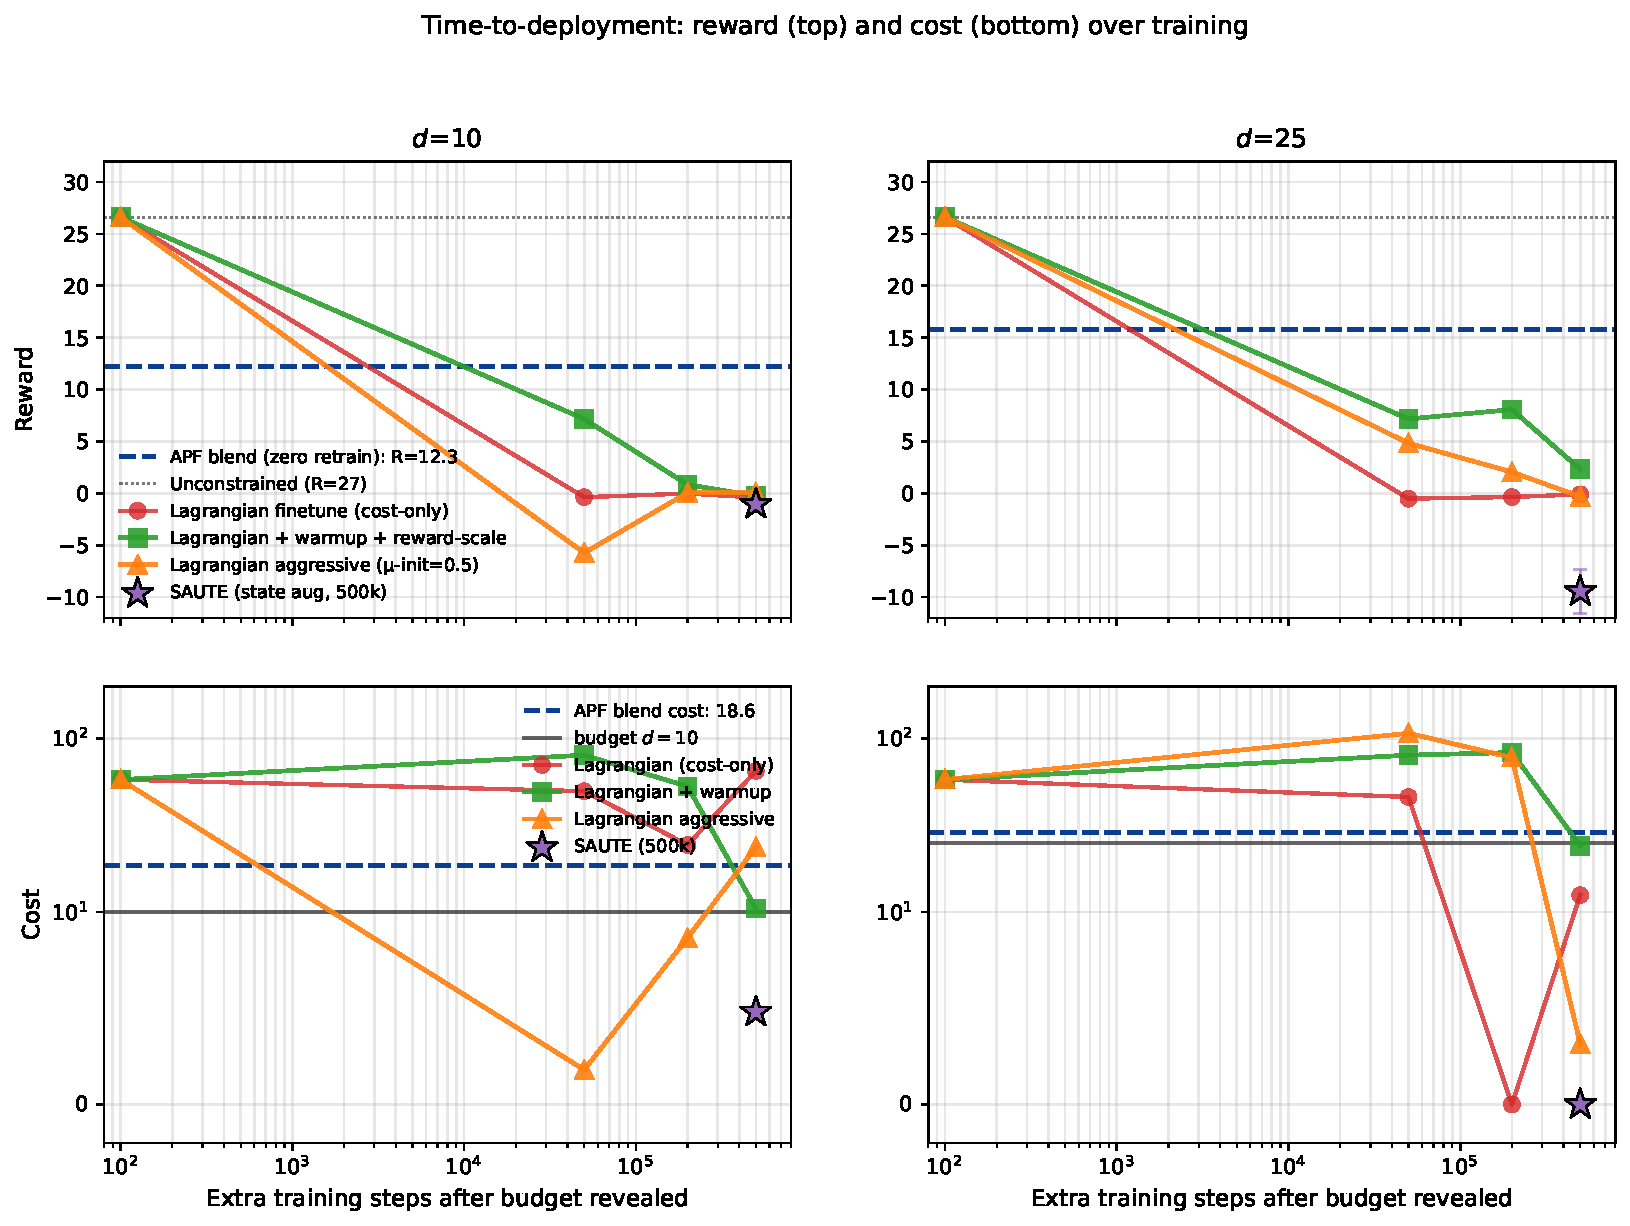
\includegraphics[width=\linewidth]{figures/fig_time_to_deployment.pdf}
    \caption{Time-to-deployment on Safety Gymnasium PointGoal1, both budgets and both axes. \emph{Top row}: reward over extra training steps. \emph{Bottom row}: cost over the same axis with budget line. Blue dashed: APF-blend reward and cost at zero retraining. Curves: four CMDP retraining variants starting from the same pretrained actor (single seed each, four hyperparameter regimes); star: SAUTE~\citep{sootla2022saute} at 500k. The blend retains higher reward than every retraining variant tested at every checkpoint, but its cost (18.6 at $d\!=\!10$, 28.6 at $d\!=\!25$) exceeds the budget; some retraining variants satisfy the budget tightly at the price of $R\!\approx\!0$. The two methods occupy different points on the reward-cost frontier.}
    \label{fig:time_to_deployment}
\end{figure}

\begin{table}[h]
\centering
\caption{Final-step ($500$k) baseline summary on Safety Gymnasium. \textbf{$\mathbb{E}[C]\!\le\!d$}: expected-cost feasibility. The APF blend dominates the retraining baselines \emph{on the reward axis} at the same compute budget. Some retraining baselines satisfy the cost constraint more tightly at the price of near-zero reward.}
\label{tab:baselines}
\begin{tabular}{lcccc}
\toprule
Method & $d$ & Reward & Cost & $\mathbb{E}[C]\!\le\!d$ \\
\midrule
\textbf{APF blend (zero retraining)} & 10 & $\mathbf{12.3}$ & $18.6$ & \textcolor{red}{$\times$} \\
\textbf{APF blend (zero retraining)} & 25 & $\mathbf{15.8}$ & $28.6$ & \textcolor{red}{$\times$} \\
\midrule
SAC-Lag default                      & 10 & $-0.41$ & $65.0$ & \textcolor{red}{$\times$} \\
SAC-Lag default                      & 25 & $-0.10$ & $12.5$ & \checkmark \\
SAC-Lag warmup + reward-scale        & 10 & $-0.24$ & $10.4$ & \textcolor{red}{$\times$} \\
SAC-Lag warmup + reward-scale        & 25 & $2.32$  & $24.1$ & \checkmark \\
SAC-Lag aggressive                   & 10 & $0.07$  & $23.6$ & \textcolor{red}{$\times$} \\
SAC-Lag aggressive                   & 25 & $-0.32$ & $3.1$  & \checkmark \\
SAUTE (state aug, uses $\rho_t$)     & 10 & $-1.0$  & $4.8$  & \checkmark \\
SAUTE (state aug, uses $\rho_t$)     & 25 & $-9.5$  & $0.0$  & \checkmark \\
\bottomrule
\end{tabular}
\end{table}

Two distinct operating regimes appear.
The post-hoc blend gives the highest reward at every compute checkpoint but violates the cost constraint in expectation at $d\!\in\!\{10, 25\}$ (it is feasible at $d\!=\!40$, Table~\ref{tab:safetygym}).
Retraining baselines either violate the budget while preserving partial reward (warmup at intermediate checkpoints) or satisfy it by collapsing reward to $\approx\!0$ (aggressive Lagrangian, SAUTE).
\textbf{Neither method dominates in the strict constrained-optimisation sense; they occupy different points on the reward-cost frontier.}
A practitioner should choose based on whether their constraint is operationally a soft pacing target (favour the blend, retain useful policy) or a hard expected-cost limit (favour SAC-Lag warmup or SAUTE, accept reward collapse).
We do not claim retraining cannot eventually reach better operating points with more compute; under the budgets we tested, the blend offers a competitive position on the reward axis with zero retraining.


\section{Derivations, Protocols, and Negative Results}
\label{app:additional}

\subsection{Boltzmann-Response Pacing Argument (Motivation)}
\label{app:proof}

Under an idealised Boltzmann response $P(\mathrm{risky}\mid\lambda)=P_0\exp(-\alpha\lambda)$, budget-rate balance $(T-t)\cdot P(\mathrm{risky}\mid\lambda) = d-C_t$ gives $\lambda=\tfrac{1}{\alpha}\ln\frac{(T-t)P_0}{d-C_t}$.
At TWAP ($u\!=\!1$), $\lambda_0=\tfrac{1}{\alpha}\ln\frac{TP_0}{d}$.
The multiplicative weight relative to TWAP reduces to $w = \exp(\alpha(\lambda-\lambda_0)) = \frac{(T-t)/T}{(d-C_t)/d} = \tau/\rho = 1/u$.
This is a motivating observation, not a guarantee: the Boltzmann assumption does not hold for trained policies.
SAUTE~\citep{sootla2022saute} identifies the same $u$ as a state-augmentation feature; the closed form here serves only as one default schedule among many monotone candidates.

\subsection{Schedule Approximation}
\label{app:approx}

\begin{figure}[h]
    \centering
    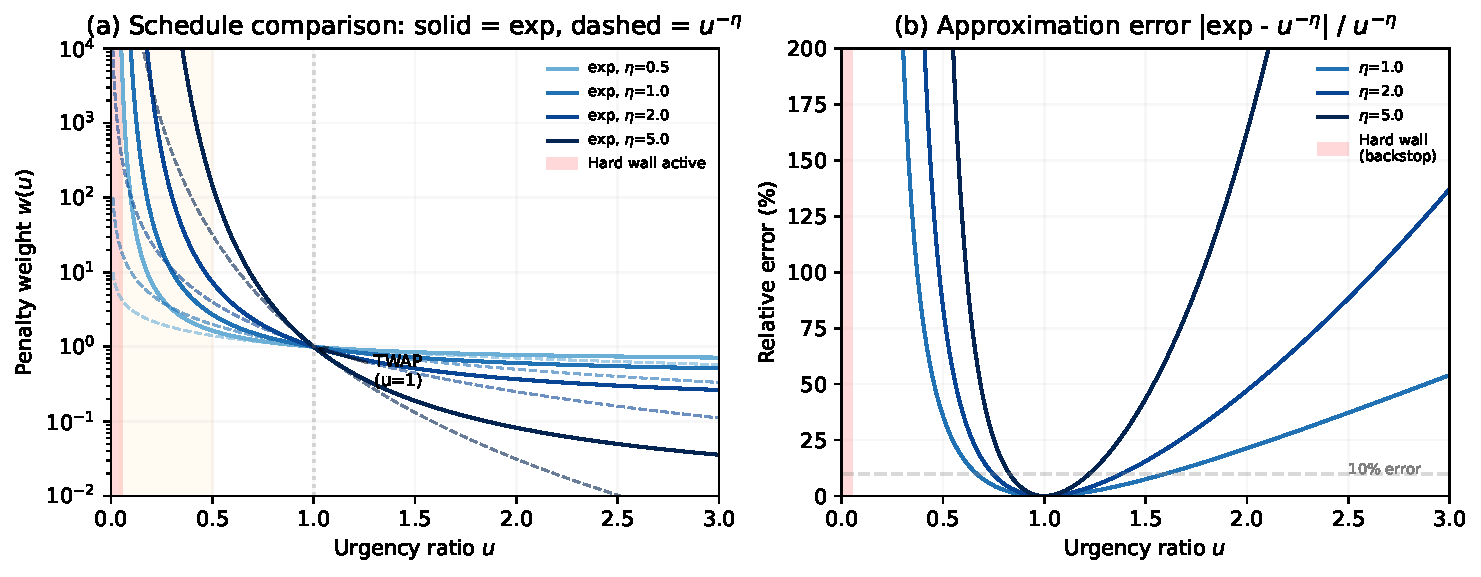
\includegraphics[width=\linewidth]{figures/fig_approx_quality.pdf}
    \caption{(a)~$\exp(\eta(1/u-1))$ (solid) vs.\ $u^{-\eta}$ (dashed). Red: $u<0.05$ hard-wall zone. (b)~Relative approximation error $<10\%$ for $u>0.5$.}
    \label{fig:approx}
\end{figure}

\subsection{Safety Controllers}
\label{app:apf}

\textbf{APF navigator (Safety Gym).}
Agent position $x$, goal $g$, hazard centres $\{h_i\}$ with radius $r$, influence distance $r_{\mathrm{inf}}$:
$F_{\mathrm{goal}}=(g-x)/\|g-x\|$, $F_{\mathrm{rep}}=k_r\sum_{i:\|x-h_i\|<r+r_{\mathrm{inf}}}(x-h_i)/\|x-h_i\|^3$, $d^\star=\mathrm{norm}(\alpha F_{\mathrm{goal}} + (1-\alpha)F_{\mathrm{rep}})$.
Mapped to body-frame action: $\mathrm{thrust}=\langle d^\star,\hat{\mathbf{e}}_{\mathrm{fwd}}\rangle$, $\mathrm{turn}=\mathrm{clip}(\Delta\theta/(\pi/2),-1,1)$.
We use $\alpha\!=\!0.5$, $r_{\mathrm{inf}}\!=\!0.6$ m, $k_r\!=\!1.0$.

\textbf{Zero-yaw / WakeAdapt (wind farm).}
$\pi_{\mathrm{safe}}(s)\equiv 0$ in normalized yaw-action space, minimising the per-turbine surrogate cost.
Deployment replaces with a precomputed table $T(\bar v,\bar\phi)\to\{y_i\}$ minimising farm-level DEL.

\subsection{Binary vs Nonlinear Cost (Wind Farm)}
\label{app:nonlinear}

\begin{table}[h]
\centering
\caption{Binary vs.\ nonlinear fatigue cost (3-turbine wind farm, 10 ep at 12--16 m/s).}
\label{tab:nonlinear}
\begin{tabular}{lccc}
\toprule
Method & Power (MW) & NegYaw & Fatigue \\
\midrule
Unconstrained                & 29.7 & $[66,75,71]$ & 20.3 \\
Binary AC ($\eta\!=\!2$)     & 28.1 & $[8,8,10]$   & 86.2 \\
Nonlinear AC ($\eta\!=\!5$)  & \textbf{29.2} & $[80,81,83]$ & \textbf{12.8} \\
\bottomrule
\end{tabular}
\end{table}

\subsection{Learned Cost Critic on Wind Farm}

\begin{table}[h]
\centering
\caption{Learned $Q_c$ on 3-turbine wind farm (10 ep). $Q_c$ trained on 100 ep with the nonlinear fatigue cost.}
\label{tab:qc_windfarm}
\begin{tabular}{lcccc}
\toprule
Method & Power (MW) & NegYaw & Fatigue & Fatigue $\times$ \\
\midrule
Unconstrained                                & $24.6\!\pm\!5.6$ & $[84,96,94]$ & 54.6 & $1.0\times$ \\
$Q_c$, $\eta\!=\!2$, gs$\!=\!0.05$           & $\mathbf{28.1\!\pm\!2.7}$ & $[43,44,43]$ & $\mathbf{9.5}$ & $5.7\times$ \\
$Q_c$, $\eta\!=\!5$, gs$\!=\!0.5$            & $28.8\!\pm\!2.0$ & $[55,54,51]$ & $10.4$         & $5.3\times$ \\
Analytical surrogate ($\eta\!=\!5$)          & $29.2$ & $[80,81,83]$ & $12.8$ & $4.3\times$ \\
\bottomrule
\end{tabular}
\end{table}

\subsection{Reward--Cost Scatter: from-scratch SAC-Lag (additional ablation)}
\label{app:fromscratch_saclag}

\begin{figure}[h]
    \centering
    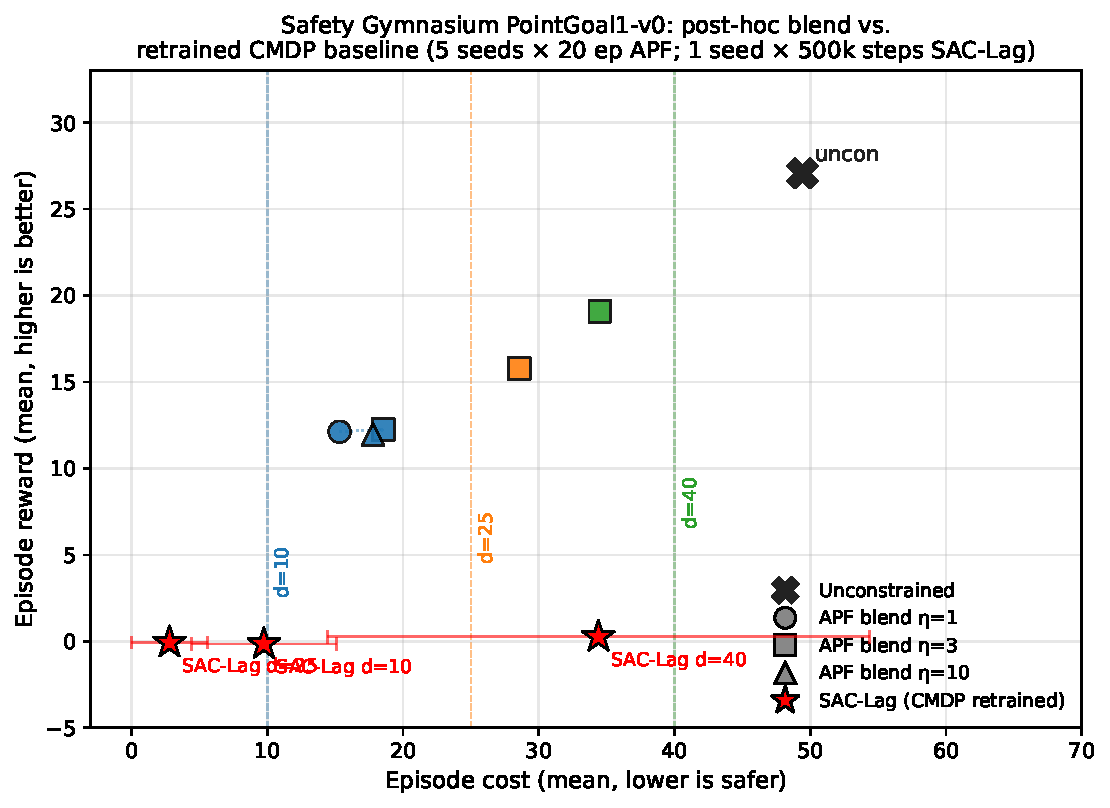
\includegraphics[width=0.75\linewidth]{figures/fig_sg_comparison.pdf}
    \caption{From-scratch SAC-Lag (red stars), 500k steps per budget, vs.\ APF blend (blue/orange/green) and unconstrained (X). Same qualitative failure mode as the from-pretrained Lagrangian finetune in Figure~\ref{fig:time_to_deployment}; the choice of warm-start does not rescue CMDP at this compute.}
    \label{fig:sg_comparison}
\end{figure}

\subsection{Nine Attempted Gradient-Variant Rescues on SG}
\label{app:sg_rescues}

When the gradient variant is forced to work on SG (low $\kappa$), the following all fail:
\begin{enumerate}[leftmargin=*]
    \item \textbf{Pessimistic $Q_c$ ensemble.} 10 heads, $\nabla_a(\bar Q+q\sigma_Q)$ with $q\!\in\!\{0,1,4\}$. $q\!=\!0$ ties or wins at every budget.
    \item \textbf{Online $Q_c$ refit.} Episode-boundary MC refit with L2 anchor; no improvement.
    \item \textbf{MPC with learned $f_\theta$ + $Q_c$.} Matches unconstrained (55 cost, 17\% sat at $d\!=\!10$).
    \item \textbf{MPC true-env + oracle cost, cost-only.} Reward collapses to $-120$; 26\% sat via "agent stuck in corner."
    \item \textbf{MPC true-env reward-weighted.} $\lambda$ (to $10^6$) dominates $\beta\cdot r$; same outcome.
    \item \textbf{MPC true-env feasibility-filtered.} Few feasible candidates; falls back to min-violation; same outcome.
    \item \textbf{Full MBRL post-hoc.} Ensemble $f_\theta$ + $Q_r$ + $Q_c$ + CEM + online refit. Cost $\approx$ uncon, reward $\approx$ uncon, sat $\approx$ uncon.
    \item \textbf{CBF 1-step kinematic.} Reward preserved, cost barely drops; 1-step insufficient for momentum.
    \item \textbf{CBF multi-step (constant-action rollout).} Errors compound; reward degrades, cost rises.
\end{enumerate}
The explicit $\pi_{\mathrm{safe}}$ blend (main body) succeeds because $\pi_{\mathrm{safe}}$ is \emph{not} constrained to lie near $\pi_{\mathrm{perf}}$'s action distribution.
When the performance policy was trained for short-path navigation, its action support does not cover the safe-corridor actions; a local gradient correction cannot reach them. An APF navigator can.

\subsection{Coupling-Strength Measurement Protocol}
\label{app:coupling_protocol}

20 episodes per domain under the frozen policy; uniform subsample of 2000 $(s,a)$ pairs; $\|\nabla_a Q_c\|_2$ and $\|\nabla_s Q_c\|_2$ via autodiff; $\kappa$ = ratio of sample means; nonparametric bootstrap with 1000 resamples for CIs.

\subsection{Retraining-Baseline Hyperparameters}
\label{app:baselines}

\textbf{SAC-Lagrangian default}: $\mu_0\!=\!0.1$, $\mu_{\mathrm{lr}}\!=\!0.005$, no warmup, no reward scaling.
\textbf{Warmup variant}: $\mu$ held at 0 for the first $50$k steps (pure-reward warmup), $\mu_0\!=\!0.05$ after, $\mu_{\mathrm{lr}}\!=\!0.005$, reward$\times 5$.
\textbf{Aggressive}: $\mu_0\!=\!0.5$, $\mu_{\mathrm{lr}}\!=\!0.05$, reward$\times 5$, no warmup.
All start from the pretrained unconstrained actor; $\alpha_{\mathrm{ent}}\!=\!0.2$ fixed.
\textbf{SAUTE}: state-augmentation with $\rho_t$, reward replaced with $-1/(1-\gamma)$ when $\rho_t\!<\!0$; otherwise standard SAC; trained from the pretrained actor for 500k steps.

\subsection{9-Turbine Zero-Shot Transfer Ablation}
\label{app:wf_9turb}

We zero-shot-transfer the pretrained 3-turbine EBT actor to the 9-turbine $3\!\times\!3$ \texttt{square\_3x3} layout (the transformer is permutation-equivariant) and re-run a subset of the ablation modes (3 seeds $\times$ 30 ep). Pure $\pi_{\mathrm{safe}}$ retains $97.8\%$ of unconstrained power, mirroring the 3-turbine result; uncon power varies $\sim\!2$ MW seed-to-seed and the wake-steering advantage of $\pi_{\mathrm{perf}}$ is not visible above this variance. The same pattern across both layouts indicates the limitation is in actor training, not farm geometry.

\begin{table}[h]
\centering
\caption{Wind-farm 9-turbine zero-shot ablation. Pretrained 3-turbine EBT actor transferred to $3\!\times\!3$ grid. Pattern matches 3-turbine: pure $\pi_{\mathrm{safe}}$ is power-competitive with uncon RL.}
\label{tab:wf_9turb}
\begin{tabular}{lcccc}
\toprule
Mode & \% Uncon power & Blend (MW) & Uncon (MW) & Seeds sat \\
\midrule
$\pi_{\mathrm{safe}}$ alone (zero yaw) & $97.8\!\pm\!1.2\%$  & 76.9 & 78.7 & 3/3 \\
const $\sigma\!=\!0.5$                  & $101.8\!\pm\!1.6\%$ & 78.0 & 76.7 & 0/3 \\
const $\sigma\!=\!0.7$                  & $103.5\!\pm\!2.5\%$ & 78.2 & 75.7 & 0/3 \\
switch $u\!<\!0.8$                      & $104.2\!\pm\!0.9\%$ & 79.2 & 76.0 & 3/3 \\
urgency $\eta\!=\!3$                    & $96.9\!\pm\!4.7\%$  & 73.9 & 76.4 & 3/3 \\
\bottomrule
\end{tabular}
\end{table}

\subsection{Path to Wind-Farm Deployment}
\label{app:deployment}

\begin{enumerate}[leftmargin=*]
    \item \textbf{DEL-calibrated cost}: replace per-turbine surrogate with a control-oriented DEL model~\citep{wes2024DEL, guillore2024sectoravg}.
    \item \textbf{WakeAdapt-equivalent $\pi_{\mathrm{safe}}$}: precompute $T(\bar v, \bar\phi)\to\{y_i\}$ minimising farm DEL.
    \item \textbf{SCADA counterfactual}: retrospective evaluation on real operational data.
    \item \textbf{Non-stationary wind}: online refit of $Q_c$ / DEL surrogate; concept-drift detection.
    \item \textbf{High-fidelity validation}: FAST.Farm calibrated to SCADA.
\end{enumerate}

\bibliography{references}
\bibliographystyle{plainnat}

\end{document}
